\documentclass[twoside,openright,a4paper,11pt,french]{article}
\usepackage[utf8]{inputenc}
\usepackage[french]{babel}
\usepackage[T1]{fontenc}
\usepackage{emptypage}

% Utilisation d'url
\usepackage{url}
\urlstyle{sf}

% Utilisation d'images, stockées dans le répertoire ./pics/
\usepackage{graphicx}
\graphicspath{pics/}

% Définition des marges
\usepackage{geometry}
\geometry{
  left=25mm,
  right=25mm,
  top=25mm,
  bottom=25mm,
  foot=15mm
}

\begin{document}

\pagestyle{plain}

% La page de garde
\thispagestyle{empty}

\begin{center}
       \noindent
       
\includegraphics[height=2.5cm]{./pics/uds.eps}       
       
       \vfill\vfill

    {\large \textsc{Licence 3 de Sciences, mention Informatique}}

    \bigskip\bigskip

    {\large \textsc{Réseaux et Protocoles}}

    \vfill\vfill

% Titre du document
    {\huge \sc
      \begin{center}
		Modèle de document\\pour un rapport d'étude
      \end{center}}

    \vfill\vfill

    {\large Présenté par}

\medskip

% Identité des auteurs
    {\large Julien \textsc{Montavont}}

% Contact mail
    {\small \url{montavont@unistra.fr}}

\bigskip

\end{center}



% La table des matières
\parskip=0pt
\tableofcontents

\newpage

\section{Introduction}
\label{sec:intro}

Dans les réseaux locaux, les machines peuvent communiquer directement les unes
avec les autres par le biais d'un lien physique.\footnote{Ce lien peut directe
de machine à machine, ou indirecte: passant par d'autre équipement (switch,
hub,...).} En revanche, établir un lien entre des machines sur des réseaux
différents n'est pas aussi facile, cela pose en effet deux problèmes majeurs:
\begin{itemize}
\item Deux réseaux différents n'utilisent pas forcement la même technologie
pour transmettre des données au niveau protocolaire ou du lien physqiue.
\item Comme les machines ne sont pas physiquement sur le même réseau, il faut
un système d'adressage afin qu'une machine puisse joindre une autre machine
située dans un réseau différent, peu importe sa localisation.
\end{itemize}
Dans le cadre d'une communication, il est souvent pratique de diviser les
fonctionnalités nécessaire à l'échange d'information.  Pour cette raison il est
utile de définir un modèle théorique pour séparer les différentes tâches.
Aujourd'hui le standard en terme de modèle de communication est le modèle OSI
({\it Open Systems Interconnection}), qui divise en 7 couches les
fonctionnalités en question.

\bigskip
Le problème relatif à l'interconnection des réseaux (vu plus haut) est traité
par la couche 3 (nommé couche réseau) du modèle OSI.
Cette couche peux être fonctionnellement mise en oeuvre par le protocole IPv4.
C'est actuellement le protocole réseau (relative à la couche 3 du modèle OSI)
le plus utilisé et qui à permit le déployement massive d'Internet dans le
monde.\\
Dans la suite de ce rapport, nous allons étudier le fonctionnement d'IPv4, les
possibilités qu'il offre et l'écosystème de protocoles qui gravitent autour
d'IPv4 et qui sont nécessaires à son bon fonctionnement.  Nous allons commencer
par explorer le contexte de création de ce protocole et comprendre les
motivations qui ont pousser le concevoir.



\section{Histoire d'IPv4}
\label{sec:hist}
% Daniel intro

Une forte demande de la part des universités et centres de recherche aux
Etats-Unis à donné lieu à la création et la mise en ouvre d'un nouveau concept
de réseau permettant d'interconnecter les différentes structures de facon
efficace afin de partager des informations, et d'autre part, de faire des
expérimentations sur les réseaux.
\\
En effet jusqu'à présent les réseaux informatiques utilisaient le même principe que les
réseaux téléphoniques: la commutation de circuits; ce qui n'était pas très 
efficace en terme de resources et de materiel\footnote {
Dans un réseau à commutation de circuits chaque péripherique pouvaient utiliser
un seul lien à la fois (ciruit). Lors d'une trasmission un lien était réservé
pour toute la durée de la communication et rendait donc le péripherique
inutilisable pour d'autre transmission vers un different destinataire (c'est le même
principe que celui des réseaux téléphoniques).
http://www.tcpipguide.com/free/t\_CircuitSwitchingandPacketSwitchingNetworks.htm .}.
\\
Pendant les années 1960 le concept de reseau à paquets commuté a été inventé et mis en 
pratiqu; d'abord dans la reseau du NPL (UK National Physical Laboratory)
puis dans l'agence americaine ARPA ({\it Advanced Research Project Agency})
\footnote {http://www.livinginternet.com/i/iw\_packet\_inv.htm}.
\\
Dans un réseau à commutation de paquets ({\it Packet Switching}), la connection
entre deux machines n'est pas continue et les données sont répartits et
envoyées en plusieurs paquets.  L'abandon d'une connexion continue a permit de
se passer de la monopolisation d'un lien (circuit) dédié ce qui a apporté la
possibilité d'avoir simultanément plusieurs connections (envoyer et recevoir
des paquets vers different destinataires, un peu comme une boite aux lettres). 
\\
Le réseau créé au sein de l'agence gouvernemental ARPA, baptisé ARPANET, est un
des premiers réseaux à fonctionner sur la base de paquets. Le principe de
communication par paquet repose sur la découpe des informations à transmettre en plus
petits paquets qui peuvent chacun prendre un chemin différent pour arriver à
destination.  Avant ARPANET, la communication réseau était basée sur la
communication par circuit électrique dont les informations étaient envoyées en
continue sur un seul lien. Dans ce sens ARPANET a posé la base à partir de 
laquelle Internet a été créé. 
\\
L'ARPA (aujourd'hui DARPA: {\it Defence Advanced Research Project Agency}) est
une agence de recherche créée par le département américain de la défense en
1957 afin de développer de nouvelles technologies à usage militaire. ARPANET,
a été conçu comme un réseau en étoile reliants plusieurs serveurs.
Chaque serveur est représenté comme un noeud et peut stocker, traiter des données ou servir de relais.
Ainsi, il existe plusieurs chemins pour accéder à un noeud et lorsqu'un de ceci
est hors service, il est toujours possible de rejoindre le destinataire
en passant par un autre chemin. En effet, une des caractéristiques les plus intéressantes
d'ARPANET a été une certaine robustesse: ARPANET ne dépendait pas d'un centre
névralgique qui aurait pu être détruit en cas d'attaque\footnote { Il faut par
contre noter que l'hypothèse qui affirme qu'ARPANET ait été construit dans le
but de créer un réseau resistant aux attaques nucléaires a été démystifié par
l'{\it Internet Society}:
http://www.internetsociety.org/internet/what-internet/history-internet/brief-history-internet
.}
\\
Ce réseau se développa pour arriver à 23 noeuds en 1971 et 111 en 1977.
Afin d'uniformiser ce réseau, Vint Cerf et Bob Kahn ont introduit la première
version du protocol TCP.  Historiquement, le protocole IP constituait la
partie de TCP qui s'occupait de la transmission en mode sans connexion.
La transmission en mode sans connexion permet l'échange de paquet sans que les
deux hôtes soient obligés d'établir une connexion auparavant.
Cette version est ce qu'on aurait pu nommer l'IPv1 et elle est documentée dans
la RFC 675. Elle fut modifiée et publiée en 1977 et correspond à la
deuxième version de TCP (IPv2). 
\\
Le protocole TCP avait donc deux fonctions: il devait premièrement
permettre une transmission fiable d'informations entre deux hôtes, et en plus
servir de protocole de routage et de packaging (partie correpondante à IP).
Cependant, pour être cohérant avec le modèle en couche, qui différencie la fiabilité
(couche transport) et le routage (couche réseau), il fut décidé en 1978 de
diviser le protocole TCP en deux protocoles distincts.\footnote {
{\it "We are screwing up in our design of internet protocols by violating the
principle of layering. Specifically we are trying to use TCP to do two
things: serve as a host level end to end protocol, and to serve as an
internet packaging and routing protocol. These two things should be
provided in a layered and modular way. I suggest that a new distinct
internetwork protocol is needed, and that TCP be used strictly as a host
level end to end protocol." } - IEN 2 (Comments on Internet Protocol and TCP)
}.
Le protocole TCP ne s'occupe maintenant plus que de la partie transport. La
partie réseau a été prise en charge par le protocole IP.  C'est finalement le
1er janvier 1983 que l'ARPANET adopte les protocoles TCP et IP (IP dans sa version 4). 


\section{Concepts et utilisation}

Des données transmisent en utilisant le protocole IPv4 sont encapsulées dans un message que
l'on appelle un paquet IPv4. Ces paquets sont constitués d'un entête suivis des données à transmettre.

% Mossi
\subsection{Adresse IPv4}

L'entête contient des informations essentielles pour la transmission d'un paquet, notamment les
adresses source et destination.

Une adresse IP sert à identifier une machine (et plus précisément une des interfaces de cette machine)
dans un réseau particulier.
Comme nous le verrons plus tard cet identifiant unique permet de désigner à la fois un
réseau et une machine précise au sein de ce réseau.
Une adresse est codé sur 32 bits ce qui permet de coder 2\^32 soit 4294967296 adresses différentes.
Par convention on peut représenter une adresse IPv4 comme une suite de 4 nombres décimaux séparés par des points,
chacun traduisant un octet. Cette représentation a contribué à simplifier l'utilisation et la manipulation
des adresses.
Comme chaque nombre représente un octet, les valeurs de celui-ci sont comprises entre 0 et 255.

\vspace{1cm}
Exemple: adresse à valeur décimale: 212.217.0.1 => correspond sous sa forme
binaire à: 11010100.11011001.00000000.00000001
\vspace{1cm}

\subsubsection{Notion de NET ID et HOST ID}
Une adresse IPv4, en tant qu'identifiant d'une machine dans un réseau, contient deux informations:
une première partie qui identifie le réseau appelé NET ID (les bits de poids fort), une seconde qui identifie l’hôte appeler host-ID (les bits de poids faible).
Les machines qui se trouvent donc sur le même réseau partage le même NET ID pour leur adresse.

La longueur de ces deux parties est variable: la taille du HOST ID dépend de la taille du NET ID. Pour représenter la longueur de ces différentes parties on a introduit la notion de masque

\subsubsection{Masque de réseau}

Le masque sert à représenter la scission entre le NET ID et le HOST ID.
Il est codé sur 32 bits et adopte la même représentation qu'une adresse IP, à savoir
4 nombres décimaux séparé par des points.
La position des bits à 1 dans le masque corresponde à la position des bits définissant le NET ID dans l'adresse IP.
Pour obtenir les bits du NET ID il suffit de faire un ET logique entre l'adresse et son masque. Tous les autres bits (donc les bits à 0)
feront donc partie du HOST ID.
Les bits à 1 sont contiguës et commencent au bit de poids fort: le nombre de bit à 1 dans le masque, donne
le nombre de bit faisant partie du NET ID en partant du bit de poids fort dans l'adresse.

En conséquence plus le nombre de bit à 1 dans le masque est grand, plus le NET ID sera grand, et plus le HOST ID sera petit, car il restera moins de bit pour définir le HOST ID (la somme des deux devant évidemment faire 32 bits).

\begin{figure}[h]
\centering
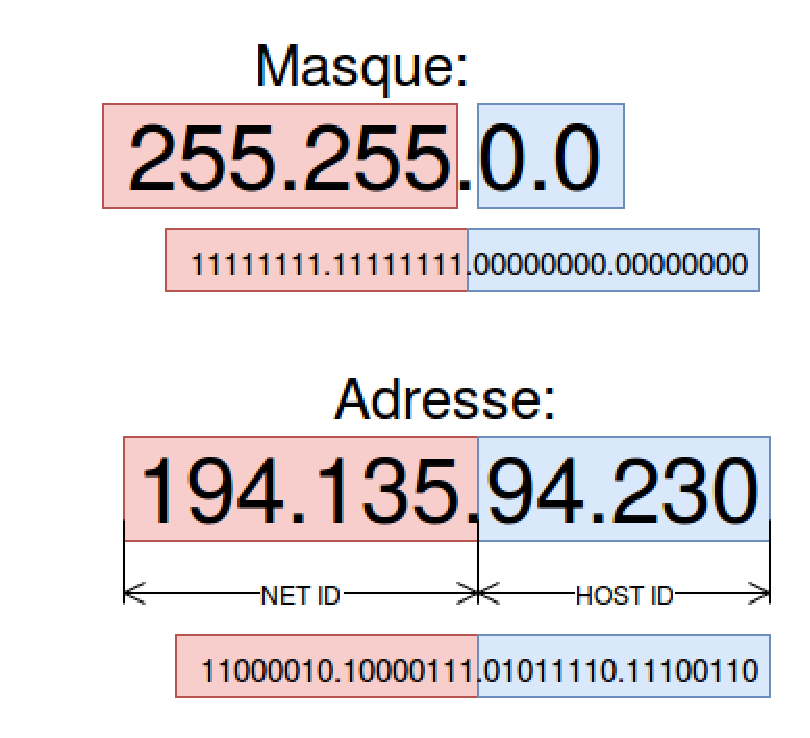
\includegraphics[width=7cm]{./pics/maskipv4.eps}
\caption{Example de masque de réseau.}
\label{fig:exmask}
\end{figure}

//TODO exemple
//TODO exemple invalide

\subsubsection{Classes d'adresse IP}
La technique de classe d'adressage IP ( classful network ) est une méthode
utilisée de 1981 à 1993 pour allouer des adresses IPV4.
Historiquement les classes d'adresse IP correspondaient à une plages d'adresses avec un masque figer pour une classe donnée.
Ce système permettait de déduire le masque en fonction
de l'adresse IP étant donné que chaque classe avait son masque défini de manière standard.
Il fut décrit dans le RFC 791\cite{url-RFC-791}.

Selon ce principe, chaque adresse IPv4 peut appartenir à une des 5 plages
d'adresses (appelées classes):

\begin{table}[h]
  \centering
% On paramètre ici le placement du texte dans les cases, en mode paragraphe de 5cm de large dans la case de gauche ("p{5cm}") et automatique avec un alignement à droite dans la case de droite ('r')
  \begin{tabular}{| p{5cm} | p{5cm} | r |}
    \hline
    \textbf{Classe} & \textbf{Masque reseau} & \textbf{Adresses}\\
    \hline
    A & 255.0.0.0 & De 0.0.0.0 a 127.255.255.255\\
    \hline
    B & 255.255.0.0 & De 128.0.0.0 a 191.255.255.255\\
    \hline
    C & 255.255.255.0 & De 192.0.0.0 a 223.255.255.255\\
    \hline
    D & 240.0.0.0 & De 224.0.0.0 a 239.255.255.255\\
    \hline
    E & Non defini & De 240.0.0.0 a 255.255.255.255\\
    \hline
  \end{tabular}
  \caption{Classes IPv4}
  \label{tab:classes}
\end{table}

A partir de ce tableau nous pouvons voir qu'il suffit de regarder les 4 bits de
poids fort pour déduire à quelle classe appartient une adresse.  Par exemple si
une machine à pour adresse 152.123.87.45 on sait en regardant les 4 premiers
bits que cette adresse fait partie de la classe B (car l'adresse commence par
10). De là, la machine n'a pas besoin de masque en plus car elle sait que le
masque correspondant un adresse de classe B est 255.255.0.0 .

Chaque classe à un certain nombre d'octets servants à identifier le réseau. Une
adresse IP de classe A à un identificateur de réseau sur 1 seul octet. Une
adresse IP de classe B sur 2 octet et une de classe C sur 3 octets.

Ce système permet donc d'adresser de nombreux réseaux avec un nombre de machine
variable en fonction de la classe, et tout cela sans avoir besoin de
communiquer ou de paramétrer un masque; celui-ci étant normalisé pour chaque
classe.  

Cependant il a un gros inconvénient, étant donné que les masques sont
figés, un réseau peut ne pas utiliser une partie plus ou moins importante
de ses adresses. Par exemple si un réseau contient 500 machines, il ne peut pas
utiliser d'adresse de classe A étant donné que celles-ci ne permettent d'avoir
que des réseaux de 254 machines maximum. Il va donc falloir utiliser des
adresses de classe B minimum, car elles permettent d'adresser 65534 machines au
sein d'un réseau\footnote{
De ce fait on remarque que la distribution de l’espace d’adressage entre
classes n'est pas homogène: la classe A a possédée 50\% de l’espace
d'adressage engendrée par les classes, la classe B 25\% , la classe C 12,5\%  et
les classes D et E 6,25\%.}. Nous pouvons donc utiliser 500 adresses sur les 65534
disponible, mais le reste sera "perdu".  Ce système était simpliste mais
n'était pas utilisable sur le long terme car il "gâche" des adresses en
n'utilisant pas tout son espace d'adressage.

Afin d'avoir un niveau supplémentaire, grâce auquel on gagne en flexibilité et
en efficacité dans l'attribution d'adresses à l'intérieur d'une classe, on a
introduit le concept de sous-réseau. Celui-ci correspond à couper la plage
d'adresses appartenant a un bloc d'une classe en plusieurs réseaux. Grâce aux
sous-réseaux on peut par exemple diviser une adresse de classe B en 256
sous-réseaux pouvant chacun avoir 256 interfaces connectées. 


\subsubsection{CIDR}

Aujourd'hui le système le plus utilisé est CIDR (Classless Inter-Domain
Routing) remplace le système de classe d'adresse. CIDR permet de créer des
masque beaucoup plus fin, étant donné qu'on n'est plus limité à des masque de
réseau fixe, on peut ajuster le masque pour avoir le nombre de machine
adressable dans un réseau le plus proche possible du nombre de machine que l'on
souhaite adressé.  Cela permet de limiter les pertes en adresse inutilisé, si
la plage est correctement découpée.  On peut donc créer des masques à la
séparation entre le NET ID et le HOST ID se trouve n'importe où, même en plein
milieu des octets (ce qui était impossible avec les classes d'adresse), ce qui
apporte une plus grande flexibilité.  Cela permet aussi de créer une hiérarchie
dans une plage d'adresse réseau qui serait découper en plusieurs réseaux
"fils", et cela permet notamment, avec cette hiérarchie, de réduire la table de
routage des routeur.  De là est né une nouvelle notation des masques: on écrit
le nombre de bit à 1 dans le masque à la suite de l'adresse IP et séparé par un
slash.


\begin{figure}[h]
\centering
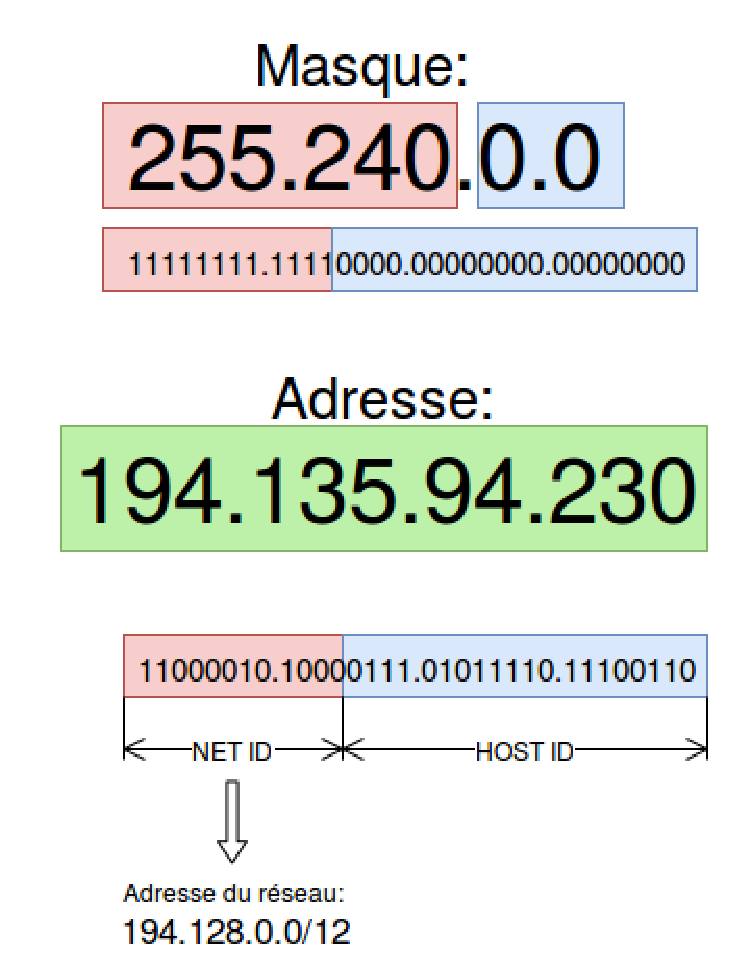
\includegraphics[width=7cm]{./pics/maskipv4cidr.eps}
\caption{Example de masque utilisant le systeme CIDR.}
\label{fig:exmask}
\end{figure}


\subsubsection{Types d'adresses}
La variété des exigences en matière de réseaux a donnée lieu à une
classification progressive des adresses selon des rôles bien précis. En effet,
pas toutes les adresses IPv4 ont la même signification: à certaines adresses
(ou plages d'adresses) ont été attribué par convention des fonctions ou des
caractéristiques particulières.  Dans la suite de cette partie nous analyserons les
adresses IP sous trois aspects différents: nous classifierons d'abord les adresses selon
le type de diffusion qu'elles permettent d'effectuer, puis nous introduirons le
concept d'adresse publique et d'adresse privée, enfin nous parlerons de l'utilisation
particulière qui a été faite avec certaines adresses.



\paragraph{Mode de diffusion}
Dans le cadre des transmissions, en plus de communiquer entre deux interfaces, il est 
parfois nécessaire qu'un message soit reçu par un groupe de machines ou que 
même la totalité du réseau reçoivent ce message.

On a défini pour cela plusieurs types de diffusions associés à certaines adresses particulières.

Le type de diffusion le plus utilisé est la diffusion en unicast. Dans ce mode,
l'adresse IP désigne une machine de manière unique. L'adresse IP appartient
à une seule machine et sert à l'identifier sur un réseau.  C'est le type
d'adresse que nous avons abordé jusqu'à présent.  Mais il peut être intéressant
de pouvoir contacter plusieurs machines en même temps. On pourrait bien sûr
envoyer des paquets en unicast à chaque machine que l'on souhaite contacter,
mais cela serait fastidieux et inonderait le réseau inutilement. Une solution plus
pratique est d'avoir une adresse qui désigne plusieurs machines à la fois. Cela
permet d'envoyer un seul paquet qui est remis à plusieurs machines. Il
existe pour faire cela plusieurs types de diffusion.
\begin{itemize}
\item Le broadcast: Ce mode de diffusion permet d'envoyer un paquet unique tout en 
joignant toutes les machines sur un réseau. Lorsque les machines reçoivent ce
paquet, elles s'aperçoivent que l'adresse de destination du paquet est l'adresse de
broadcast et elles vont alors traiter le paquet. L'adresse de broadcast d'un réseau
est défini comme la plus "haute" adresse du réseau: cela se traduit par la mise
à 1 de tous les bits de la partie HOST ID. Cette adresse ne peut donc pas être
attribuée à une machine en tant qu'adresse unicast.  Le broadcast est utilisé
par des protocoles tel que ARP et DHCP.  Nous pouvons remarquer qu'avec cette
définition, nous pouvons envoyer un message de broadcast à n'importe quel
réseau, incluant le notre. En réalité (sauf
configuration volontaire) les routeurs ne laissent pas passer les messages de
broadcast d'un réseau à un autre; excepté quelques cas spéciaux comme DHCP où un
serveur peut s'adresser à plusieurs réseaux, et où ses messages de broadcast
peuvent être relayés par les routeurs (appelés DHCP agents).
\item Multicast: Ce mode de diffusion permet d'envoyer un paquet à destination
de plusieurs machines. L'adresse IP multicast sera donc vu comme l'adresse d'un groupe
mutlicast, qui désigne donc plusieurs machines. Pour qu'une machine fasse partie d'un
groupe multicast, il faut qu'elle s'abonne à ce groupe: cela veut dire que si elle reçoit
un paquet avec comme adresse de destination l'adresse du groupe multicast, elle va traiter
le paquet.
Bien entendu les membres d'un même groupe ne sont pas obligés d'être sur le même réseau. Dans ce
cas les machines doivent indiquer à leur routeur qu'il existe un ou plusieurs groupe multicast et celui-ci deviendra alors un routeur multicast 
 Le protocole IGMP va entrer en jeu pour faire cet échange.
Cette indication a été rendu obligatoire dans le but de ne pas faire circuler tous les paquets a destination de groupes multicast.
 Il n'est en effet pas nécessaire de relayer tous les paquets de tous les groupes
multicast sur le réseau, si celui-ci ne contient aucun abonné au groupe.
Le faite d'avertir le routeur qu'il y a des machines abonnées à un groupe dans le réseau permet aussi à celui-ci
d'établir un lien avec l'émetteur. Mais ceci fait partie du routage des paquets par le routeur.
Il existe une plage d'adresse qui est réservée pour les adresses IP multicast. Lorsqu'on veut contacter
plusieurs machines, une adresse dans cette plage peut être utilisée.
Elle s'étend de l'adresse 224.0.0.0 à l'adresse 239.255.255.255 et a pour masque 240.0.0.0 . Cela laisse donc 2\^28 adresses
multicast différentes.
Au sein de cette plage d'adresse il existe une catégorisation:
//TODO
\begin{itemize}
\item
\end{itemize}
Ce mode permet de limiter le nombre de paquets envoyés pour joindre plusieurs machines et il est très utilisé dans le cas
de diffusions en streaming ou de vidéoconférences, où il faut faire parvenir une même information à plusieurs participants.

\item Anycast: Une adresse anycast, tout comme les adresse multicast, identifient plusieurs machines. La différence avec multicast
est qu'en mode de diffusion anycast, la paquet ne va pas être remit à tous les membre du groupe, mais seulement à un seul (le premier qui le réceptionne).
Le choix de la destination et le routage à adopter se base sur plusieurs critères telles que la "distance" avec la machine, la disponibilité,
la charge, ... . Cela permet d'avoir des systèmes toujours disponible même en cas de forte charge, en repartissant celle-ci sur
plusieurs machines.
\end{itemize}



\paragraph{Adresses publiques et adresses prive}
L'expansion exponentielle d'Internet a posé, seulement quelques années après sa création, des
soucis de pénurie d'adresses. Plusieurs mesures ont été prises pour limiter la
portée de ce problème. Malgré ça, le stock d'adresses IPv4 non réservée
est malheureusement épuisé depuis le 2011.

Une des dispositions les plus connues et efficaces a été la création du concept
d'adresses privées. Le RFC 1918 introduit la notion d'adresses privées: une adresse
appartenant à cet catégorie est un identifiant unique dans un réseau (ou sous
réseau) mais il ne comporte aucune contrainte d'unicité dans l'échelle globale
(Internet). L'idée derrière la conception des adresses privées était celle d'
avoir des identifiants qui peuvent être utilisés lorsque une machine n'a pas
pas besoin de communiquer avec des interfaces au-delà de son réseau.

A ce titre des plages d'adresses ont été réservées pour cet usage:

\begin{itemize}
\item Un bloc d'adresses appartenant a la classe A: \textbf{10.0.0.0/8}
\item 16 blocs d'adresses appartenant a la classe B: \textbf{172.16.0.0/12}
\item 256 blocs d'adresses appartenant a la classe C: \textbf{192.168.0.0/16}
\end{itemize}

\smallbreak
Le concept d'adresses privées s'oppose à celui d'adresses publiques: ce dernier est 
une adresse unique sur Internet et est en conséquence atteignable par n'importe
quel hôte sur Internet.

Aujourd'hui des systèmes comme celui de la NAT ({\it Network Address
Translation}) permettent à des machines ayant des adresses IP privée de communiquer
de manière transparente avec des hôtes en dehors de leur réseau. Ce système est
largement utilisé dans les réseaux domestiques pour permettre aux machines au
sein de ceux-ci d'être directement connecté à Internet. On parlera plus en
détail du NAT dans la section %TODO \ref{} %.
\smallbreak


 
L'augmentation des difficultés relatives à la procédure de réservation des adresses
publiques au sein des organisme responsables des allocations\cite{url-RFC-1918}
(tels que le IANA) ont contribués a promouvoir l'utilisation des adresses privées à la place
 des adresses publiques lorsque cela est possible.
L'utilisation des adresse privées a pour conséquence la préservation des plages
d'adresses IP publiques, ce qui constitue un avantage certain: l'utilisation
des adresses privées permet d'éviter le gaspillage des adresses publique là ou elles
ne sont pas nécessaires.


\paragraph{Adresses speciales}
L'usage spéciale d'une adresse IP découlait de l'émergence
%TODO (apparition??) 
d'un nouveau besoin dans le domaine des réseaux; c'est pour
ça que jusqu'à 2002, l'attribution des rôles spéciaux des adresses
IPv4 était présentés dans divers document, qui présentaient, et répondaient à chaque fois à une
problématique bien particulière. Le RFC3330 est un des premiers documents à
rassembler les classification des adresses IPv4 selon leur rôles et significations.

%TODO lien%

\begin{description}
\item[0.0.0.0/8]
Cette plage d'adresses indique la machine courante dans le réseau courant.
Les adresses dans cette plage sont notamment utilisées dans certains protocoles de
configuration comme adresse source, lorsqu'une machine n'a pas encore d'adresse effective.
%RFC 1122 %

\item[127.0.0.0/8]
Une adresse appartenant a ce bloc est dénommée adresse de {\it loopback}.  Un
paquet envoyé vers une telle adresse retourne directement chez l'expéditeur, sans sortir
du contexte de la machine émettrice. Parmi les adresses de cette plage,
127.0.0.1 est celle utilisée le plus fréquemment\footnote{Comme l'indique
le RFC 1122, certaines implémentations de l'adresse de {\it loopback} se
limitent à utiliser le bloc 127.0.0.1/32, ce qui se traduit par l'unique utilisation de
l'adresse 127.0.0.1 }: dans plusieurs contextes cet adresses est référencée par
l'alias "{\it localhost}".\footnote{La correspondance entre le nom {\it localhost} et
l'adresse 127.0.0.1 est généralement mise en place par le système d'exploitation.
Dans les systèmes de type UNIX une entrée reliant ces deux entités est généralement
présente dans le fichier "/etc/hosts".}
Une adresse de {\it loopback} n'a pas de sens en dehors
d'une interface même, et c'est pour cela qu'elle ne devrait apparaître à aucun moment dans le réseau.

%RFC 1122 %

\item[169.254.0.0/16]
Cet plage d'adresses a été désignée comme contenant les adresses qu'on appelle
de {\it lien local}.  Les adresses dites de {\it lien local} sont utilisée lorsqu'une 
machine n'a aucun moyen d'obtenir une adresse IP (par exemple par le biais
d'un serveur DHCP ou simplement avec une configuration manuelle).  L'obtention
d'une adresse de {\it lien local} est faite de façon automatique à travers un
processus d'auto-configuration souvent appelé par l'acronyme APIPA ({\it
Automatic Private Internet Protocol Addressing}) ou par le nom IPv4LL.  Le
fonctionnement du processus APIPA (décrit dans le RFC 3927) est assez complexe
 et entraîne l'utilisation de certaines fonctionnalités du
protocole ARP (qu'on traitera plus en détail dans la section %TODO \ref{sec:suiteproc} % )
. Son fonctionnement peut être synthétisé dans ses grandes lignes par la démarche suivante:

\begin{description}
\item[Sélection de l'adresse]
La machine choisit aléatoirement
    \footnote{Il est conseillé d'utiliser l'adresse MAC de l'interface en question
    pour générer l'adresse de {\it lien local} pour qu'il y ait une plus forte chance
    qu'elle soit unique dans le réseau.} 
une adresse appartenant à la plage 169.254.0.0/16

\item[Sondage sur l'adresse]
Une fois qu'on a sélectionné une adresse, il faut s'assurer que la même adresse ne soit
pas déjà utilisée par d'autres machines sur le réseau. Dans ce but la machine
pose la question à toutes les autres machines du réseau au moyen d'un ou plusieurs messages
en brodcast, et attend une réponse pendant un certain intervalle de temps\footnote{
Des précautions sont prises pour éviter les conflits générés par plusieurs
machines qui effectuent simultanément cette action pour la même adresse,
notamment: des intervalles de temps aléatoires entre l'envoie des messages et la mise
en place d'une écoute active des autres messages pendant le temps de l'enquête.}
L'absence de réponse indique que l'adresse est bien unique. Si l'adresse n'est
pas unique il faut en choisir une autre.

\item[Annonciation de l'adresse]
A ce point la machine peut communiquer aux autres machines l'adresse qu'elle
vient de réserver.

\end{description}



Ce processus est basé sur le concept de {\it Zeroconf}: il permet la mise en
place d'un réseau IPv4 sans aucune configuration. Ce type de système,
C'est aussi grâce a ce genre de systèmes, qu'on 
pourrait synthétiser par la devise %TODO slogan??  
"plug and play", que le concept de Networking (et avec lui Internet) a pu se
diffuser assez rapidement: grâce à APIPA un réseau IPv4 peut être facilement
mis en place sans le besoin d'aucune connaissance technique.\\

La plage d'adresses 169.254.0.0/16, désigne une plage d'adresse privée: les
adresses de type {\it lien local} ne sont donc pas atteignables en dehors de
leur réseau de définition. 
Cette plage d'adresses pose par contre des limites par rapport aux autres
plages d'adresses privée car, à la différence des autres, elle ne peut pas être
divisée en sous réseaux\footnote{Ce qui est assez logique si on considère que
le processus d'obtention d'une adresse de {\it lien local} (APIPA) utilise
les liens "physiques" entre les machines pour communiquer, et il ne peut
 considérer aucune notion de sous-réseau.}
: en effet un paquet destiné à une adresse de {\it lien local} ne doit pas être
retransmise par un hôte intermédiaire.\footnote{Dans le paquet destiné
a une adresse de {\it lien local} le champ TTL est usuellement mis a 1
pour empêcher des forwarding.}

\item[192.88.99.0/24]
Les adresses appartenant à ce bloc désignent des routeurs 
fournissant un service de type {\it 6to4}. Ce type de service
permet de relier des réseaux IPv4 avec des réseaux IPv6.
Les adresses dans cette plage sont traitées comme étant des adresses
de type {\it anycast}.


\end{description}




% Luigi Coniglio 
\subsection{En-tête IPv4}
Dans un paquet IPv4, les données utiles sont précédées par un en-tête ayant une longueur minimale de 20 octets 
(dans les cas où aucune option supplémentaire n'a été spécifiée).
La figure suivante montre le contenu de l'en-tête d'un paquet IPv4.

\begin{figure}[h]
\centering
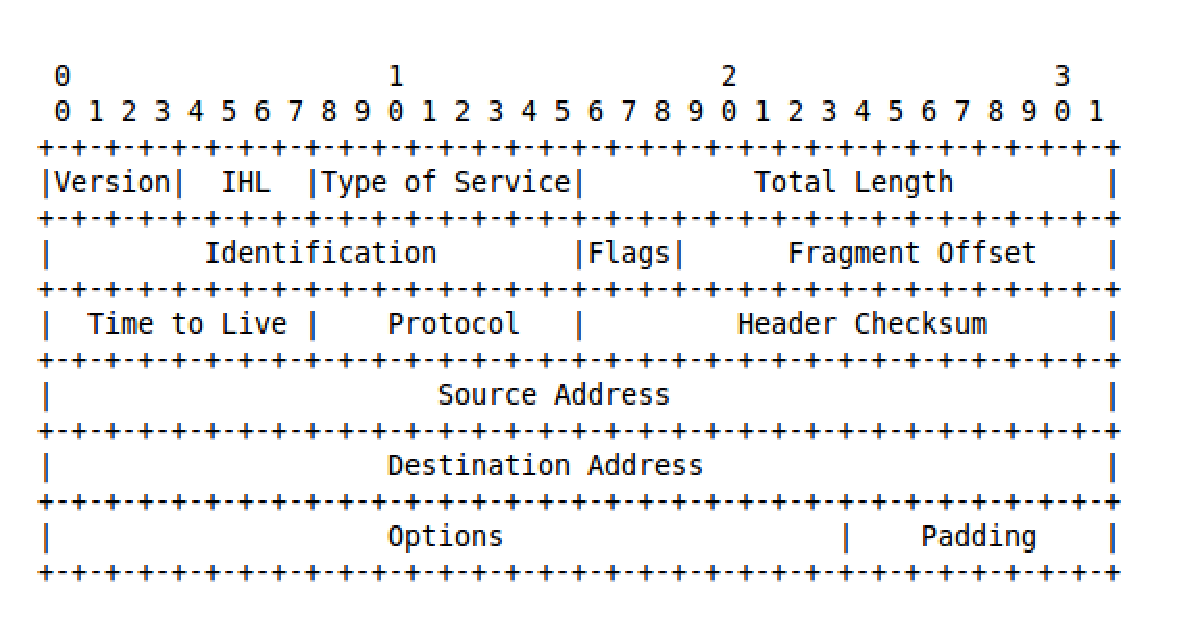
\includegraphics[width=12cm]{./pics/IPv4header.eps}
\caption{En-tete IPv4.}
\label{fig:entipv4}
\end{figure}


Comme on peut le voir sur la figure ci-dessus, un en-tête IPv4 est composé, en plus du padding, de
13 champs. En réalité nous verrons plus loin que cet en-tête
peut, quand c'est nécessaire, contenir un champ additionnel grâce auquel
on peut spécifier quelques options qui ne sont pas présentes dans les 13 champs
au dessus.


Commençons par voir en détail les 13 champs d'un en-tête IPv4 standard:

\begin{description}
\item [Version] 
Ce champ occupe les 4 premiers bits de l'en-tête IPv4.\\
Il est utilisé pour déterminer le type de protocole utilisé par la couche
réseau (couche 3). Dans le cas d'IPv4 ce champs contiendra la valeur
4, qui identifie le protocole IPv4.

Ce champ n'est pas positionné par hasard dans l'en-tête. En effet, pour
connaître la position des autres champs de l'en-tête, il faut d'abord savoir
quel est le protocole utilisé et donc le type de l'en-tête.
En pratique, dans la plupart des cas ce champ n'est pas très utile, car le
protocole à utiliser pour la couche 3 est souvent spécifié dans l'en-tête du
protocole de la couche liaison.

\item [IHL]
Le champ IHL (acronyme de Internet Header Length) spécifie la taille de l'en-tête IPv4. 
Bien entendu, en disant cela on souligne un concept important du protocole IPv4: 
la taille de l'en-tête n'est pas fixe.

La taille de l'en-tête est exprimée en blocs de 32 bits. Étant donné une taille de
4 bits pour le champ IHL, la longueur maximale d'un en-tête IPv4 est de 15 blocs de
32 bits, ce qui correspond à 60 octets. Comme l'en-tête IPv4 a une taille minimale
de 20 octets (160 bits), le champ IHL ne peut pas contenir une valeur inférieure à 5.

\item [Type of Service]
Le champ Type of Service, mieux connu sous l'acronyme ToS, est utilisé pour 
spécifier la qualité de service souhaité pour l'envoie d'un paquet IPv4.
Ce champ occupe un octet de l'en-tête et il est composé de trois parties.
Une première partie de 3 bits permettant d'indiquer la priorité avec laquelle
le paquet doit être traité, les 3 bits suivants sont utilisés pour spécifier 
certaines caractéristiques du service, notamment: le temps, le débit et la fiabilité.
Enfin, les deux derniers bits n'ont pas été utilisés et leur signification a été 
réservée pour des implémentations futures.

En réalité l'histoire de ces champs est bien plus longue et complexe,
car en pratique la façon d'utiliser ces champs a été modifiée plusieurs fois au 
cours du temps.
\footnote{L'utilisation des 8 bits du champ ToS a été redéfinie
par cinq standards différents (plus divers standards expérimentaux).
Les documents présentant ces standards sont mentionnés dans le chapitre 
"Historical Definitions for the IPv4 TOS Octet" du RFC 3168}
Ce manque de stabilité a parfois causé une certaine confusion lors des différentes implémentations.
\footnote{Comme le souligne le RFC 3260 {\it "At least one implementor has expressed confusion about the
relationship of the DSField, as defined in RFC 2474, to the use of
the TOS bits, as described in RFC 1349"}}

Aujourd'hui les 8 bits du champ ToS sont utilisés par le mécanisme DiffServ
(Differentiated Services). Ce système utilise les 6 bits premiers du champ
ToS (DSCP - Differentiated Services Code Point) pour marquer chaque paquet
comme appartenant à un niveau de priorité et à une classe de service. Chaque
classe détermine le type de traitement que doivent effectuer les routeurs sur le paquet qui le traverse
 (PHB - Per-Hop behaviour), toutefois le service offert
par chaque routeur est fortement lié à sa configuration.
\footnote {
{\it "The DiffServ standard does not specify a precise definition of "low," "medium,"
and "high" drop probability. Not all devices recognize the DiffServ (DS2 and
DS1) settings; and even when these settings are recognized, they do not
necessarily trigger the same PHB forwarding action at each network node. Each
node implements its own response based on how it is configured."} - 
Implementing Quality of Service Policies with DSCP
http://www.cisco.com/c/en/us/support/docs/quality-of-service-qos/qos-paquet-marking/10103-dscpvalues.html}
Les 2 derniers bits du champ ToS sont utilisés pour l'extension ECN ({\it Explicit Congestion
Notification }). Cette extension, proposée par le RFC2481n et introduite deux années plus tard par le RFC3168,
ajoute un système de contrôle de la congestion du trafic réseau. Dans le cas d'une saturation
du réseau, ce champ est utilisé pour notifier ce problème et demander au dispositif émetteur
une réduction du rythme auquel les paquets sont envoyés, afin de réduire l'attente et
la perte de paquets.

\item [Total length]
Comme le suggère son nom, ce champ est utilisé pour indiquer la taille totale du
paquet IPv4: en-tête + données. Le champ {\it Total length} est défini sur 16
bits, ce qui permet d'indiquer une valeur comprise entre 0 et 65 535 octets. Comme l'en-tête
est compris dans la longueur totale d'un paquet, cette valeur ne sera jamais inférieure
à 20 (taille minimale d'un en-tête IPv4 en octets).
Le RFC 791 impose à tous les dispositifs d'un réseau IPv4 la capacité de recevoir
des paquets d'une taille maximale de 576 octets, cette prérogative permet d'éviter une fragmentation excessive.

\item [Identification]
Ce champ (sur 16 bits) permet d'identifier les fragments appartenant au même paquet.

\item [Flags]
Les 3 bits du champ Flags sont utilisés pour gérer la fragmentation d'un paquet.
Un de ces bits est utilisé pour indiquer si le paquet peut être fragmenté ou
non. Ce bit, appelé DF ({\it Don't Fragment}), doit être pris en considération
par les routeurs sur le chemin du paquet pour décider si un paquet est trop grand pour être
transmit, s'il doit être retransmit sous forme de fragments plus petits ou s'il doit être rejeté. 
Un autre bit, appelé MF ({\it More Fragments}), indique si le paquet est suivi 
par d'autres fragments. Le bit MF est mis à 0 dans le dernier fragment ou dans
les paquets qui n'ont pas été fragmentés.

Un des trois bits de ce champs n'est pas utilisé actuellement mais il a été
réservé pour de possibles applications futures.
\footnote {Ce bit a aussi été le protagoniste d'un des plus connu poissons
d'avril de l'IETF. Pour faciliter les tâches des systèmes de filtrage 
le RFC 3514 propose d'utiliser ce bit pour étiqueter les paquets malveillants et à ce
titre tous les paquets étant envoyés avec ce bit (renommé "{\it Evil Bit}") 
mis à 1 seraient mis à la poubelle.}

\item [Fragment Offset]
Lorsqu'un paquet a été fragmenté, cet en-tête est utilisé pour déterminer la
position (offset) d'un fragment par rapport à l'ensemble du paquet réassemblé.
Le décalage de chaque fragment est exprimé en blocs de huit octets (ou 64
bits). Le champ Fragment Offset utilise 13 bits de l'en-tête IPv4, ce qui permet
un offset maximale de 65528 octets.\footnote {En pratique un tel offset n'est
jamais utilisé car, en ajoutant un en-tête minimale de 20 octets, la taille
totale du paquet réassemblé dépasserait la longueur maximale d'un paquet IPv4.}
Étant donné que le flag MF ({\it More Fragments}) doit être mis à zéro lorsqu'un paquet 
n'est pas fragmenté, ou si il est le dernier fragment d'un paquet plus grand, 
l'unique différence entre ces deux types de paquets est la valeur du 
champ Fragment Offset qui, dans le cas d'un paquet non fragmenté, est
toujours zéro.

\item [Time to Live]
Ce champ détermine le nombre maximal de fois qu'un paquet peut être retransmit. 
Il est utilisé pour empêcher qu'un paquet puisse être retransmit à l'infini.
Chaque routeur le long du chemin d'un paquet regarde la valeur du champ. Si celle-ci
a atteint 0, il détruit le paquet, et sinon il décrémente le champ par le
nombre de secondes que le paquet passe en attente avant qu'il soit transmis.

En théorie, le TTL indique le nombre de secondes pendant lesquelles un paquet
peut continuer à être retransmis dans un réseau, mais un routeur 
 décrémente toujours ce champ d'au moins 1 (même si le paquet a été
retransmis en moins d'une seconde) et, en considérant les performances des routeurs
d'aujourd'hui, le TTL indique en pratique le nombre maximum de routeur qu'un paquet
 peut traverser au cours de son acheminement.

L'espace réservé au TTL dans l'en-tête IPv4 est d'un octet, ce qui veut dire qu'on a un 
TTL maximum de 255.\footnote {Le RFC 1700 recommande une valeur par défaut de 64.}

Quand un paquet a été détruit suite à l'expiration du TTL, le routeur qui a
détruit le paquet peut décider d'envoyer un message d'erreur à l'émetteur du
paquet détruit. Ce type de message (ICMP Time exceeded) est également utilisé comme
outil par {\it traceroute} pour découvrir, approximativement, le chemin 
d'un paquet IP.

\item [Protocol]
Chaque paquet IPv4 spécifie le protocole utilisé par les données transmises:
cela est l'objectif de ce champs de 8 bits 

\item [Header Checksum]
Ce champ contient une somme de contrôle et est utilisé pour détecter des 
erreurs dans l'en-tête IPv4. La valeur de ce champ est recalculé à
chaque retransmission\footnote {Cela est nécessaire car le TTL est décrémenté
à chaque retransmission et un changement de l'en-tête amène à une valeur différente
dans la somme de contrôle}: si la somme de contrôle ne correspond pas avec celle 
présente dans l'en-tête du paquet, celui-ci est détruit.


\item [adresse source et adresse destination]
Les adresses de chaque paquet IPv4 (soit l'adresse source et l'adresse de
destination du paquet) sont représentés sous forme d'une suite de 32 bits.

L'adresse source de chaque paquet représente dans la plupart des cas
l'adresse logique\footnote {Il ne faut surtout pas oublier la différence entre
une adresse physique, comme par exemple une adresse MAC (qui est liée a
l'hardware et est donc unique pour chaque machine), et une adresse logique,
comme par exemple une adresse IP (qui peut changer et identifie une machine
dans un réseau en particulier).} de la machine qui a envoyé le paquet
(à laquelle il faudra donc éventuellement répondre).  Dans certains cas,
 cette adresse ne correspond pas à celle de la machine qui a envoyé
le paquet, c'est par exemple ce qui se passe dans une requête, {\it ARP probe}
%TODO to correct: 0.0.0.0 symbolise la machine actuelle%
lorsque la valeur de l'adresse de la machine source est 0.0.0.0 (ce qui représente
une adresse indéfinie\footnote {La signification de l'adresse 0.0.0.0
est liée à la façon dont elle est utilisée. En général elle indique {\it aucune
adresse en particulier}. 

Dans la plupart des cas, cette adresse est utilisée
pour indiquer une de ces valeurs: l'adresse de la machine courante (c'est
l'adresse de loopback), n'importe quelle adresse ou le réseau (c'est le cas de la
route par défaut dans une table de routage), une adresse indéfinie ou bien une
combinaison des possibilités précédentes (c'est le cas d'une requête {\it ARP
probe} ou bien d'une requête {\it DHCP Discovery} ou {\it DHCP Request}, où
 l'adresse source 0.0.0.0 indique une adresse indéfinie mais aussi l'adresse
de la machine actuelle, qui par ailleurs n'est pas encore défini...).}
) car elle n'a pas encore déterminée son adresse IP. 

L'adresse de destination d'un paquet IPv4 identifie la machine vers
laquelle le paquet doit être expédié. Comme dans le cas de l'adresse source,
 l'adresse de destination peut aussi contenir des valeurs spéciales. En effet, certaines 
valeurs peuvent être utilisée par exemple pour identifier plusieurs machines
(adresses multicast), toutes les machines d'un réseau (adresse de broadcast) ou
la machine actuelle (adresse de loopback).

Une description plus détaillée des mécanismes liées aux adresses IPv4 est
proposée dans le chapitre  
%TODO mettre chapitre% 
de ce rapport.


\item [Options] 
Ce champ n'est pas obligatoire et il peut donc ne pas être présent dans un
en-tête IPv4. La présence de ce champ est déterminé par la valeur de
l'IHL: lorsque cette valeur indique une taille de l'en-tête IPv4 supérieure à 
la taille minimale (20 octets), l'en-tête contient des options.
Étant donné qu'un en-tête IPv4 peut avoir une taille maximale de 
60 octets (la valeur du IHL est égal à 15), le champ Options peut occuper
40 octets au maximum.

Ce champ a été conçu pour étendre les possibilités d'IPv4 en ajoutant des fonctions
supplémentaires.  Aujourd'hui il y a quelques dizaines d'options qui ont été
spécifiées\cite{url-optsIPv4} (si on considère également les options expérimentales)
mais peut d'entre elles sont réellement utilisées. Parmi les options les plus connues
on retrouve par exemple des ajouts utiles à l'administration et au debuggage
d'un réseau, comme {\it Record route} qui permet d'enregistrer les adresses
des routeurs dans le chemin d'un paquet IP, et {\it Timestamp} qui permet de
savoir le temps passé entre chaque saut du chemin.

Parmi les options il en y a deux qui ont une fonction spéciale: EOL 
({\it End Of Option List}) et NOP ({\it No Operation}): l'option EOL 
est utilisée pour indiquer la fin de la chaîne d'options, NOP est une option
sans aucun effet, elle est utilisée comme remplissage pour aligner les options 
quand elles ne sont pas alignées sur 4 octets\footnote {On rappelle que 
le champ IHL indique la longueur de l'en-tête IPv4 en blocs de 32 bits 
(4 octets)}.



\item [Padding] 
Le padding ne contient que des zéros et est utilisé quand la fin de l'en-tête
n'est pas aligné sur 32 bits (4 octets). Bien entendu, ce champ est optionnel:
en effet, il est seulement nécessaire lorsque l'en-tête IPv4 termine avec
une option dont la limite n'est pas alignée sur 32 bits. Un en-tête d'un paquet IPv4 
de 20 octets (donc sans aucune option) n'a besoin d'aucun Padding car il est aligné sur
4 octets (20 étant un multiple de 4).
\end{description}


%Victor
\section{Suite de protocoles}
\label{sec:suiteprot}

\subsection{ARP} ARP (Address resolution protocol) est un protocole à cheval
entre la couche 2 et la couche 3 permettant de faire la conversion entre les
adresses de niveau 2 et de niveau 3. Il fut décrit dans le RFC 826\cite{url-RFC-ARP}.
Il est très utilisé étant donné que les hôte connaissent souvent les adresses
IP de leur destinataire, mais rarement l'adresse de niveau 2 de ce destinataire
ou de la passerelle à contacter pour joindre le destinataire.

\subsubsection{Cache ARP} Le cache ARP ou table ARP est une table stockée en
local par un hôte et qui ressence les associations entre adresses IP et adresses
MAC.  Ces associations peuvent être soit de type statique, donc écrite "en dur"
par l'administrateur, ou dynamique, donc issue d'échange de trame ARP, et qui
possèdent en plus, par rapport associations statique, une durée de validité, étant
donné qu'une interface peut changer d'adresse IP et qu'il faut maintenir la
table à jour.  Cette table peut donc être représentée comme une suite d'entrées,
contenant chacune une adresse IP, une adresse MAC et éventuellement une durée
de vie.

\subsubsection{Fonctionnement} Prenons l'exemple où un hôte A veux envoyer un message à
un hôte B. A connaît l'adresse IP de B. Donc A va préparer le paquet qu'il va envoyer
à B, avec son adresse IP en source et l'adresse IP de B en destination. Le
paquet passe dans la couche liaison, il va être empaqueté dans une trame de
niveau 2. Cette trame aura comme adresse source l'adresse de niveau 2 de A.
A ce moment là, il ne peux pas compléter l'adresse destination de la trame: en
effet, il ne connaît l'adresse de niveau 2 du destinataire. La paquet reste
bloqué en couche 2 et ne peux pas être envoyé au destinataire. Comment obtenir
l'adresse de niveau 2 du destinataire?  Le protocole ARP est capable de faire
cette translation.

Pour faire cela l'hôte A va tout d'abord regarder dans sa table ARP si il n'a
pas une entrée pour l'adresse IP à laquelle il souhaite envoyer son paquet. Si
il trouve une correspondance, il va utiliser l'adresse MAC stockée en
correspondance avec l'adresse IP recherchée.  Si il ne trouve pas de
correspondance il va émmetre un paquet ARPREQUEST pour tenter de contacter le
possesseur de l'adresse IP qu'il souhaite contacter. Il va mettre dans ce
paquet (en plus de l'entête de niveau 3) un entête ARP. Celui-ci contient entre
autre les adresses de niveau 2 et 3 de la source et du destinataire qui sont
essentiels pour faire la résolution d'adresse, ainsi qu'un champ qui spécifie
si le paquet est un ARPREQUEST ou un ARPREPLY. 

\smallbreak
L'hôte A va donc mettre son
adresse IP en IP source (entête ARP) et son adresse MAC dans l'adresse physique
source (entête ARP). Dans le champ d'adresse IP destination (entête ARP) l'hôte
A va mettre l'adresse IP de l'hôte qu'il veut contacter. Etant donné qu'il
cherche à avoir l'adresse physique de l'hôte B, il ne peut pas indiquer
d'adresse de niveau 2 dans le champ d'adresse physique destinataire. Ce champ
est donc rempli avec la valeur 0 (entête ARP).  Sachant que l'hôte A n'a pas
l'adresse physique du destinataire, il va envoyer sa trame en broadcast pour
espérer atteindre l'hôte B sans connaître son adresse MAC. 
\smallbreak
Si l'hôte B reçoit
la requête ARP, il va analyser son entête et remplir sa table ARP avec
l'adresse IP de l'hôte A et l'adresse physique de A contenu dans l'entête ARP.
Cela permet de créer une correspondance entre l'adresse IP et l'adresse de
niveau 2 de A, pour non seulement pouvoir répondre à sa requête ARP, mais en
plus pouvoir contacter A dans le futur sans avoir besoin de refaire de requête
ARP. Ensuite l'hôte B va répondre avec un paquet ARPREPLY. L'entête est
similaire aux ARPREQUEST, seul le champ indiquant s'il s'agit d'un paquet
ARPREQUEST ou ARPREPLY change. Dans ce paquet, l'hôte B va placer son adresse
IP dans le champ adresse IP source et son adresse physique dans le champ
d'adresse physique source de l'entête ARP. Il va aussi mettre l'adresse IP de A
dans le champ adresse IP destination et l'adresse MAC de A dans le champ
d'adresse physique destination (entête ARP).  Il va ensuite envoyer ce paquet
en unicast à A.  Lorsque A reçoit le paquet ARPREPLY, il va à son tour mettre
dans sa table ARP, la correspondance entre l'adresse IP source et l'adresse de
niveau 2 source de l'entête ARP (soit les adresses de B).  Une fois cette
association mise en place, le paquet IP que voulait envoyer A au début et qui a
été mis en pause le temps que le protocole ARP fasse l'association, est enfin
envoyé étant donné que A à maintenant l'adresse physique de B.


\subsubsection{ACD} Le protocole ACD (Adresse conflict detection) permet, comme
son nom l'indique, de détecter les conflits d'adresse, qui sont l'utilisation
de la même adresse IP par deux ou plusieurs hôtes en même temps. Pour ce faire
il utilise le protocole ARP avec une succession d'étape permettant de garantir
l'utilisation de manière unique d'une adresse IP. Il fut décrit dans le RFC
5227\cite{url-RFC-ACD}.
\smallbreak
Pour commencer, ACD intervient au moment où une interface reçoit une adresse IP
(soit par DHCP, soit par une configuration manuelle,...). Il faut à ce moment
vérifier si l'adresse proposée n'est pas déjà utilisée par un autre hôte sur le
réseau.  L'hôte va alors émettre une requête ARP en broadcast en remplissant
l'entête ARP avec son adresse de niveau 2 dans le champ d'adresse physique
source et 0.0.0.0 dans l'adresse IP source (car il n'a pas encore d'adresse IP
attribuée, et pour éviter de corrompre les tables ARP des autres hôtes). Le
champ adresse IP destinataire (entête ARP) est complété avec l'adresse que l'on
souhaite acquérir. On ne peut pas remplir le champ d'adresse physique
destinataire de l'entête ARP étant donné qu'on ne sait pas si il y a des hôte
avec cette adresse déjà configurée.  Une requête ARP contenant 0.0.0.0 comme
adresse IP source est appelée ARP probe car elle sert à "sonder" si un autre
hôte utilise déjà l'adresse que l'on passe dans le champ adresse IP
destinataire.

\smallbreak
Après avoir attendu un temps pouvant aller jusqu'à 1 seconde, l'hôte va envoyer
un nombre d'ARP probe compris entre 1 et 3, et tous espacé d'un intervalle
compris entre 1 et 2 secondes.  Si dans un délai de 2 secondes après l'émission
de l'ARP probe l'hôte reçoit un paquet ARP request ou reply avec comme adresse
IP source (entête ARP) l'adresse qu'il souhaite acquérir, alors cela veut dire
qu'un autre hôte est déjà entrain d'utiliser cette adresse. L'ARP reply peut
être la réponse à un des ARP probe émis et l'ARP request peux simplement être
une demande ARP faite par l'hôte qui utilise déjà l'adresse que l'on souhaite
acquérir. En plus de surveiller ces deux types de messages, l'hôte doit
vérifier les message ARP probe qu'il reçoit. En effet, il se peut qu'un autre
hôte décide de configurer son interface avec la même adresse au même moment.
Sachant que ni l'interface de l'hôte que l'on souhaite configuer, ni
l'interface de l'autre hôte n'a encore d'adresse IP attribuer, aucune ne va
répondre à l'ARP probe émise respectivement par l'autre hôte. Cela va conduire
à l'attribution de la même adresse pour plusieurs interfaces. Pour éviter ce
problème l'hôte doit surveiller les ARP probe qui passe à son interfaces. Si il
en reçoit un avec comme adresse IP destination (entête ARP) la même adresse
qu'il souhaite acquérir mais avec une adresse physique (de l'entête ARP)
différente de la sienne, cela veux qu'un autre hôte souhaite utiliser la même
adresse que lui. Dans ce cas l'adresse IP ne peut pas être utilisée de manière
sûr.

\smallbreak
Si après les 2 secondes d'attente du dernier ARP probe, l'hôte n'a pas reçu
d'ARP probe, ou d'ARP request/reply indiquant un conflit d'adresse, alors
l'hôte peut considérer que l'adresse qu'il souhaite utiliser est unique dans le
réseau, et qu'il peut l'utiliser de manière sûr.

La dernière étape est d'annoncer que l'hôte utilise l'adresse qu'il vient
d'acquérir.  Pour ce faire l'hôte va émmettre en broadcast deux ARP
Announcement à 2 secondes d'intervalle.  Ces messages sont semblable à des ARP
probe à la seule différence que l'adresse IP source et destination (de l'entête
ARP) sont remplies avec l'adresse que vient d'acquérir l'hôte.  Le but étant de
créer une entré dans la table ARP des autres hôtes sur le réseau avec l'adresse
que vient d'acquérir l'hôte avec son adresse adresse de niveau 2. Cela permet
d'assurer que les autres hôtes auront bien la nouvelle adresse de niveau 2
associer à l'adresse IP au cas où celle-ci était attribué à une autre interface
dans le passé.

\smallbreak

Dans un deuxième temps, ACD va être utilisé en permanence durant l'utilisation
d'une adresse IP dans la mesure où lorsque que la l'interface va recevoir un
paquet ARP, elle va analyser si l'adresse IP source de l'entête ARP correspond
à une de ces adresses, et si cela est la cas et que l'adresse de niveau 2
source de l'entête ne correspond à son adresse de niveau 2, alors cela veut
dire qu'un autre hôte utilise la même adresse IP. Il y a donc un conflit
d'adresse.  Pour résoudre ce problème, l'hôte peut réagir de différente
manière:
\begin{itemize}
\item Il cesse d'utiliser l'adresse IP en question.
\item Si l'hôte doit pour quelque raison que ce soit garder son adresse IP, par
exemple si il utilise une connection TCP, alors il peut "défendre" sa
possession de l'adresse IP, seulement si il n'a pas reçu d'autre paquet ARP
portant à conflit dans les 10 dernières secondes.  Il va pour cela noter le
temps auquel il a reçu le paquet posant un conflit d'adresse et émettre un ARP
Announcement en donnant son adresse de niveau 2 en association avec l'adresse
IP dans l'entête ARP. Il va envoyer ce paquet à destination de son adresse IP,
pour signaler à l'hôte qui utilise aussi cette adresse qu'il y a un conflit
d'adresse. Cependant il peut y avoir une boucle sans fin si les deux hôtes
utilisant la même adresse se renvoient alternativement des ARP Announcement
pour défendre leur adresse. Pour éviter ce scénario, si plusieurs paquet ARP
posant un conflit d'adresse sont détecté dans les 10 dernières secondes (d'où
l'importance de noter le temps où l'hôte à reçu les paquets posant problème),
alors l'hôte cesse d'utiliser son adresse pour éviter de rentrer dans une
boucle sans fin d'échange d'ARP Announcement.
\item Si l'hôte à été configuré pour garder son adresse IP (par exemple si
c'est un routeur ou un serveur) alors l'hôte va défendre son adresse
indéfiniment.
\end{itemize}


%-------------------------------------------------------------------------------------

\subsection{ICMP} ICMP (Internet Control Message Protocol) est un protocole de
niveau 3 faisant partie intégrante du protocole IPv4. Il fut initialement
décrit dans le RFC 792\cite{url-RFC-ICMP}.
Il permet de transmettre des informations de contrôle et d'erreur. Les messages
ICMP sont empaquetés dans des paquets IP, ils disposent donc d'un entête de
paquet IP. Cet entête est le même que pour tout les autres entêtes de paquet
d'IPv4. Deux champs sont intéressant dans le cas d'un paquet ICMP, les champs
Protocol et Type of service. Le champ Protocol est mis à à la valeur 1 pour
dire que le paquet contient un message ICMP, et le champ ToS est mis à 0
//TODO(pourquoi 0?)//.  Après le header du paquet IPv4, commence la partie data
qui contient le message ICMP. Ce message contient des champs différent en
fonction du type de message à passer. Cependant les trois premier champs sont
toujours les mêmes.


\begin{figure}[h]
\centering
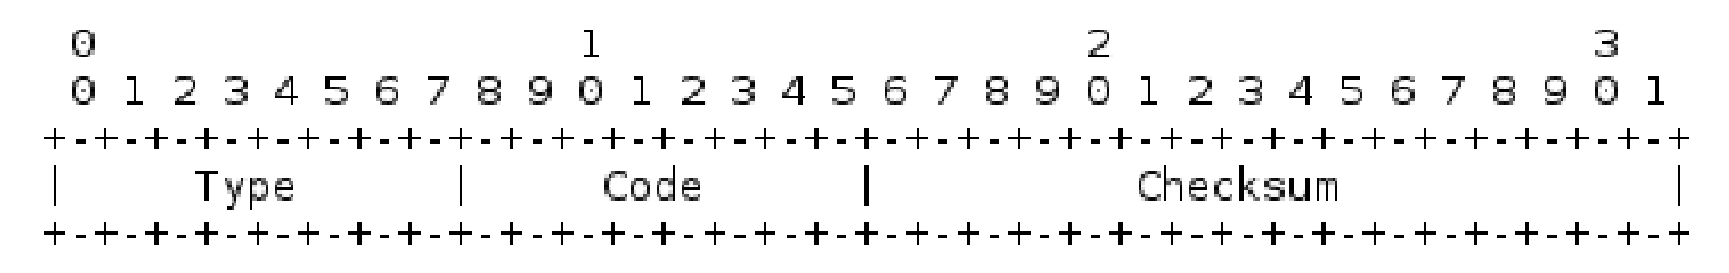
\includegraphics[width=12cm]{./pics/header.eps}
\caption{Champs de l'entête communs à tous les types de message ICMP}
\label{fig:headicmp}
\end{figure}

Le premier champ est celui de type. Il permet, premièrement, de donner le type
du paquet et de l'information à transmettre, et deuxièmement de préciser la
nature des champs qui vont suivre. En effet, comme vu plus haut, les messages
contiennent des champs différents selon le type du message ICMP.  Le deuxième
champ est le code. Il permet de subdiviser le type en donnant des détails plus
précis. Enfin le troisième champ est la somme de contrôle (checksum).
Commençons avec les messages qui possèdent l'ensemble de champs le plus simple.

\begin{figure}[h]
\centering
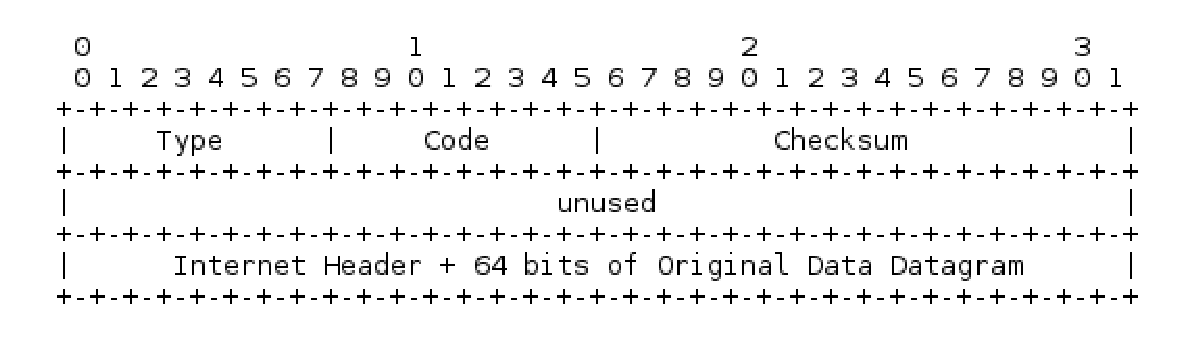
\includegraphics[width=12cm]{./pics/header1.eps}
\caption{Entête des messages de type 3 et 11}
\label{fig:head1icmp}
\end{figure}

Les messages qui utilisent cette organisation sont les messages de type 3 et
11.  Le champ Internet header contient l'entête du paquet qui a provoqué
l'envoie du message ICMP, plus les 64 premiers bits suivant le header. Cela
permet à l'émetteur de retrouver quel paquet à posé problème.

\vspace{1cm}
\textbf{Message de type 3: Unreachable Destination}
Les messages de type 3 sont émis lorsqu'un paquet n'a pas réussi à joindre la
destination (Unreachable destination). Cette erreur peux être dut à plusieurs
facteurs, et les codes permettent de préciser pourquoi le paquet n'a pas pu
rejoindre sa destination.

\paragraph{Code 0: Network Unreachable} Ce code indique que le réseau que
l'hôte essaye d'atteindre n'est pas joignable; ceci étant dut à l'absence de
route vers ce réseau.

\paragraph{Code 1: Host Unreachable} Ce code indique que le réseau à été joint,
mais que le routeur sur ce réseau n'arrive pas à joindre l'hôte à qui délivrer
la trame.

\paragraph{Code 2: Protocole Unreachable} Ce code indique que l'hôte à été
joint, mais que le protocole utilisé n'est pas actif.

\paragraph{Code 3: Port Unreachable} Ce code indique que l'hôte à été joint,
mais que le port utilisé en couche transport n'est pas actif et ne peux donc
être utilisé pour communiquer.

\paragraph{Code 4: Fragmentation needed} Ce code indique que la taille du
paquet dépasse le MTU (Maximum Transmission Unit) et que le flag DF à été mis à
1 dans l'entête IP.  En règle général, si un paquet est plus grand que le MTU,
il doit être fragmenté par le routeur pour être transmis en plusieurs paquets
plus petit. Mais comme le flag DF (Do not Fragment) est mis à 1, le paquet ne
peux être fragmenté. Le routeur émet donc un paquet ICMP de code 4.

Ces codes ont été définis dans la RFC 792, mais depuis d'autre RFC ont ajouté
des codes en plus qui sont utilisés dans des cas plus précis.

\vspace{1cm}
\textbf{Message de type 11: Time Exceeded}
Ce message est envoyé lorsque le TTL d'un paquet à atteint 0. Une autre
utilisation des ces messages est lorsque que le temps de ré-assemblage des
fragments d'un paquet est dépassé. Ces deux cas sont distingué par le code. Ces
messages ont pour destinataire l'hôte qui à envoyé le paquet qui à provoqué
l'erreur.%TODO(vérifier).

\paragraph{Code 0:}
Le code 0 est utilisé pour indiquer que le TTL du paquet posant problème est
arrivé à 0.  Lorsque le TTL d'un paquet arrive à 0, celui-ci est supprimé et un
message ICMP de type 11 et de code 0 est envoyé par le routeur qui à détecté le
problème. Cela permet principalement d'éviter qu'un paquet entre dans une
boucle et qu'il soit relayé à l'infini.

\paragraph{Code 1:} Le code 1 est quant à lui utilisé pour indiquer que l'hôte
n'a pas réussi à réassembler les fragments du paquet IP original dans la limite
de temps prévue à cet effet.


\vspace{1cm}
\textbf{Message de type 5: Redirect Message} Les message de type 5 utilisent
l'entête ci-dessous et servent à faire de la redirection. En effet, lorsqu'un
routeur détecte que le prochain routeur dans lequel va transiter le paquet se
trouve dans le même réseau que l'émetteur de ce paquet, il va envoyer un
message ICMP pour avertir cet hôte (et dans certain cas tous les hôtes sur le
réseau de l'émetteur) qu'il existe un chemin plus court en envoyant directement
les paquets vers le prochain routeur. Ce message ICMP va avoir pour effet de
modifier la table de routage interne à l'émetteur (et dans certain cas tout les
hôtes présent sur le réseau de l'hôte). Concernant le paquet que le premier
routeur à reçu, il va le transmettre vers sa destination.


\begin{figure}[h]
\centering
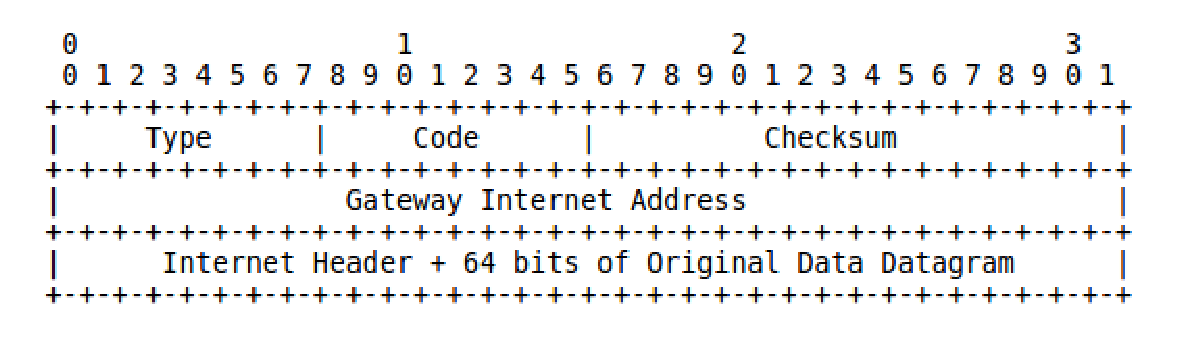
\includegraphics[width=13cm]{./pics/header2.eps}
\caption{Entête des messages de type 5}
\label{fig:head2icmp}
\end{figure}
Le champ Gateway Internet Address contient la l'adresse du routeur auquel il
faut faire transiter le trafique directement pour avoir un chemin de routage
plus court.  Le champ Internet Header contient toujours l'entête du message
ayant provoqué l'envoie du message ICMP plus les 64 bits suivant l'entête. Cela
permet à (aux) hôte(s) de pouvoir modifier leur table de routage en fonction la
destination que cherchait à atteindre le paquet.

\paragraph{Code 0}
Ce code indique que la redirection est adressée à tout les hôtes présent sur le
réseau de l'émetteur du paquet.

\paragraph{Code 1}
Ce code indique que la redirection est adressée à l'émetteur du paquet.

\paragraph{Code 2}
Ce code indique que la redirection est adressée à tout les hôtes présent sur le
réseau de l'émetteur du paquet et aux services.

\paragraph{Code 3} Ce code indique que la redirection est adressée à l'émetteur
du paquet et aux services.

Les messages de code 2 et 3 vont agir sur les services, notamment sur le ToS.

\begin{figure}[h]
\centering
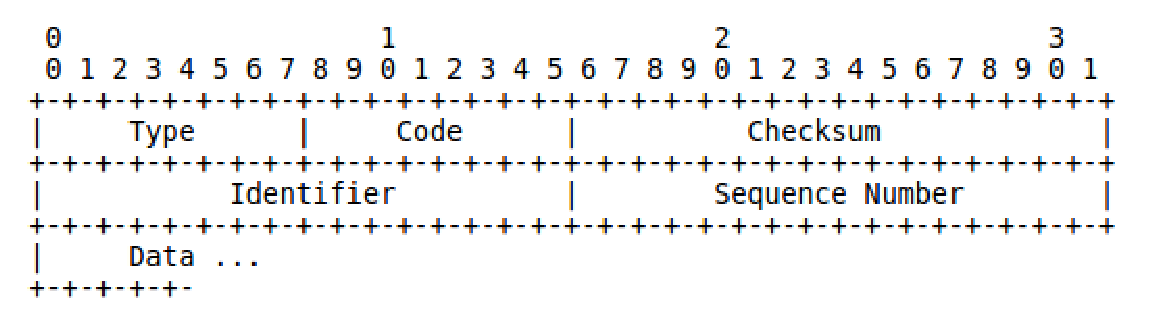
\includegraphics[width=13cm]{./pics/header3.eps}
\caption{Entête des messages de type 0 et 8}
\label{fig:head3icmp}
\end{figure}

\vspace{1cm}
\textbf{Message de type 8 et 0: Echo Request et Reply} Les messages de type 8
et 0 servent à faire des envoies et des renvoies d'information. Ils utilisent
pour cela l'entête ci-dessus. Les messages de type 8 font des envoies
d'informations, appelé echo request. Tandis que les messages de type 0 sont
envoyés en réponse aux echo request et renvoient les informations reçus de
ceux-ci; ils sont appelés echo reply. Etant donnée que les echo reply sont des
réponses aux echo request, l'adresse IP destination des echo reply est
l'adresse IP source des echo request. Ces deux messages peuvent être envoyés et
reçus aussi bien par un hôte que par un routeur. Ce sont notamment les messages
envoyés par la commande {\it ping} qui permettent de vérifier si l'on peux
communiquer avec un hôte ou un routeur.  Les champs Identifier et Sequence
Number aide l'émetteur de l'echo request à associer les echos request qu'il à
envoyés avec les echos reply qu'il à reçus.

\vspace{1cm}
Il y a bien d'autre types et code défini par ICMP, cependant ils sont plus
spécifiques ou devenu obsolètes.


%----------------------------------------------------------------------------------

\subsection{IGMP}
Le protocole IGMP est un autre protocole faisant partit intégrante d'IPv4. Il
permet en effet aux hôtes de communiquer aux routeur mutlicast leur abonnement
à des groupes multicast.  IGMPv2 et IGMPv3 sont les versions les plus utilisées
actuellement. Elles sont respectivement décrient dans le RFC
2236\cite{url-RFC-IGMP2} et RFC 3376\cite{url-RFC-IGMP3}.  Les messages IGMP
sont divisées en trois groupe:
\begin{itemize}
\item Membership Query: Les requêtes d'adhésion: servant aux routeurs pour
faire une demande aux hôtes des groupes auxquels ils sont abonnés.
\item Membership Report: Les rapports d'hôte sur leurs abonnements.
\item Leave Group: Message annonçant l'arrêt d'un abonnement d'un hôte.
\end{itemize}
Tout ces messages sont envoyés avec un TTL de 1, pour éviter que ceci ne
passent d'un réseau à un autre.

\smallbreak
IGMP va donc permettre aux routeurs d'apprendre les groupes d'abonnements des
hôtes qui sont sur le ou les réseaux du routeur. Le routeur dispose d'une liste
des groupes multicast auxquels les hôtes d'un réseau sont connectés, et ceci
pour tout les réseaux auxquels il est connecté.  Pour commencer, le routeur va
envoyer à l'adresse 224.0.0.1, deux (par défaut) Membership Query général à 30
secondes d'intervalles (par défaut).

\smallbreak
Lorsqu'un hôte reçoit un Membership Query, il va initialiser un timer pour
chaque groupe multicast auxquels il appartient. Ces timers sont initialisés
avec un temps aléatoire dont la borne supérieur est spécifié dans le Membership
Query. Ce système de timers permet de ne pas saturer le réseau avec touts les
message IGMP de tout les groupes qui seraient envoyé au même moment.  Lorsque
le timer d'un des abonnements arrive à 0, alors l'hôte émet, en multicast au
groupe en question, un Membership Report.  Si l'hôte reçoit un Membership
Report et que le timer du groupe concerné par le message reçus n'a pas encore
atteint 0, alors l'hôte va arrêter le timer. En effet le routeur sera aux
courant de l'existence du groupe car il aura reçu le même rapport que l'hôte.

\smallbreak
Le protocole IGMP est conçu pour que le routeur sache à quels groupe multicast
sont abonnés les hôte sur les réseaux auxquels il est relié. Cependant le
protocole n'a pas du tout été conçu dans l'optique de fournir la liste des
hôtes avec leurs abonnements.  C'est pour cela qu'une fois que le routeur est
au courant de l'existence d'un groupe, les autre hôtes faisant partie de ce
groupe n'envoie pas de rapport pour ce groupe.

\smallbreak
Lorsque le routeur reçoit un Membership Report il va ajouter le groupe à sa
liste de groupe présent sur le réseau auquel il est connecté. Il va à ce moment
initialiser un timer à 135 secondes (valeur par défaut).  Si il reçoit d'autre
Membership Report pour un groupe existant alors le timer est remis à sa valeur
initiale (de 135 secondes).  Lorsqu'un hôte rejoint un nouveau groupe, il va
émmetre un Unsolicited Membership Report pour s'annoncer dans le groupe, et
ainsi informer le routeur de l'existence de ce groupe ou de la remise à la
valeur initiale du timer.

\smallbreak
Le dernier cas de figure est lorsqu' un hôte veut se désabonner d'un groupe: il
va donc arrêter de traiter les messages à destination du groupe multicast. Si
l'hôte est le dernier de son groupe alors il va envoyer un Leave Group à
l'adresse 224.0.0.2.  Si il n'est pas le dernier, il peux simplement ne rien
faire et se désabonner du groupe, il ne sera plus concerné par les messages à
destination du groupe. Etant donné qu'il y a d'autres membres dans le groupe
ceci s'occuperont de "maintenir le groupe en vie".  En revanche si l'hôte ne
sais pas si il est le dernier hôte dans le groupe rien ne l'empêche d'envoyer
un Leave Group.

Lorsque le routeur reçoit un Leave Group, il sais qu'un membre à quitté le
groupe. Ce qui l'intéresse est de savoir si il y a encore des membres dans le
groupe en question ou si s'est le dernier membre qui vient de quitter le
groupe. Il va pour cela envoyer deux Membership Query spécifiquement au groupe
en question. Si aucune réponse n'est reçut le groupe est considéré comme
n'ayant plus de membre et il est oublier du routeur.  Si jamais les hôte
n'annonçait pas leur retrait du groupe (comme cela à été évoqué plus haut) et
qu'il n'y avait plus d'hôte faisant partit du groupe, alors le groupe serait
considéré sans membre et oublié lorsque le timer du routeur arriverait à 0 pour
le groupe en question.

\smallbreak
Le dernier point pour que tout cela fonctionnent, est qu'il faut que le routeur
envoie régulièrement des Membership Query général pour qu'il maintiennent à
jour sa table des groupe présent sur le réseau, sinon ceux-ci serait oublier
une fois le timer arrivé à expiration.

%----------------------------------------------------------------------------------------


\subsection{DHCP}
Le protocole DHCP (Dynamic Host Configuration Protocol) sert à l'auto-configuration
des interfaces. Plus précisément, il  permet d'attribuer une adresse IP à une
interface et de lui faire parvenir d'autres information essentielle pour le
fonctionnement de l'interface sur le réseau. La version initiale de DHCP fut décrite
dans le RFC 1531\cite{url-RFC-DHCP1}, mais cette version fut rendue obsolète par un autre
RFC, lui même rendue obsolète par le RFC 2131\cite{url-RFC-DHCP2} qui est la dernière version non
obsolète. Voyons comment une interface peut ce configurer auprès d'un serveur DHCP.

\begin{figure}[h]
\centering
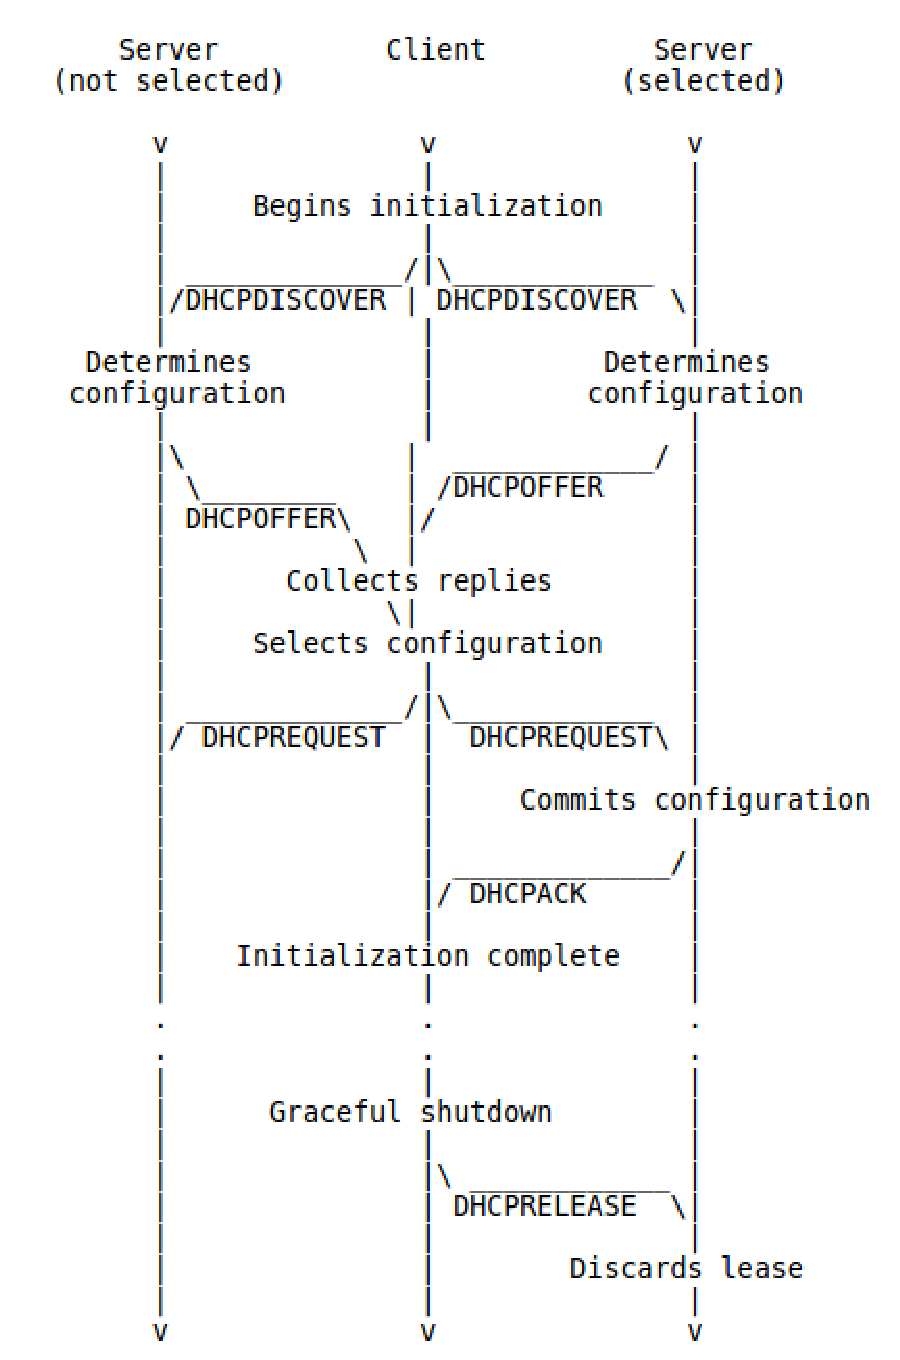
\includegraphics[width=6cm]{./pics/timeline_dhcp.eps}
\caption{Déroulement de la négociation DHCP}
\label{fig:timelinedhcp}
\end{figure}

Lorsqu'une interface, qui n'a pas d'adresse IP, souhaite en recevoir une, elle
va émettre un message DHCPDISCOVERY en broadcast sur son réseau. Des agents DHCP
peuvent faire passer
ce message DHCP sur un autre réseau si le serveur DHCP (qui distribue les
adresses) ne se trouve pas sur le même réseau que l'hôte qui fait la demande.
L'hôte va utiliser comme adresse IP 0.0.0.0.

\smallbreak
Etant donné que le message est envoyé en broadcast, tout les hôtes sur le
réseau vont recevoir le message, et en particulier le ou les serveurs DHCP qui
pourraient s'y trouver. Si cela est le cas, ceux-ci vont répondre avec un
DHCPOFFER. Ce message contient entre autre l'adresse IP proposé pour le client
souhaitant se configurer, ainsi que le masque du réseau. A ce
moment là l'adresse n'est pas encore attribuée et réservée pour l'hôte étant
donnée qu'il peut refuser l'offre et accepter l'offre d'un autre serveur. Si
jamais l'hôte ne reçoit aucun DHCPOFFER, il va ré-émettre un DHCPDISCOVERY. Si
il reçoit un ou plusieurs DHCPOFFER, l'hôte va devoir choisir une configuration
parmis celles qui lui sont proposées. Une fois ce choix fait, il va informer les serveurs DHCP de
son choix à l'aide d'un message DHCPREQUEST émis en broadcast. Ce message va
contenir l'identifiant du serveur DHCP retenu ainsi que la configuration
souhaité par l'hôte (adresse IP et masque du réseau). Ce message peut être
interprété de deux manières différentes selon le serveur:
\begin{itemize}
\item Si ce n'est pas le serveur retenu, il considère le message comme une
déclinaison de l'offre.

\item Si c'est le serveur retenu, il va sortir l'adresse attribuée à l'hôte de la
plage d'adresse libre pour ne plus l'attribuer à un autre hôte. Il va ensuite
émmettre un message DHCPACK contenant la configuration effective de l'hôte avec
notamment: l'adresse IP, le masque du réseau, la durée du bail, l'adresse
de la passerelle par défaut et l'adresse du serveur DNS.  Si pour quelque
raisons que ce soit le serveur n'est pas capable d'attribuer l'adresse proposée dans l'offre
(par exemple si l'adresse à été attribuée entre temps), le serveur émet un
DHCPNAK pour avertir l'hôte que l'adresse n'est plus disponible. L'hôte devra
alors recommencer la procédure pour obtenir une configuration.
\end{itemize}

\smallbreak
Enfin si le serveur ne reçoit pas de message DHCPREQUEST, la procédure
s'arrêtera à ce moment et l'adresse n'étant pas encore attribuée à l'hôte elle
reste disponible pour être attribuée à d'autre hôte. 

\smallbreak
Arrive la dernière étape.
Si l'hôte reçois un message DHCPACK, il peux prendre en compte la
configuration (adresse IP, masque du réseau, DNS, passerelle par défaut et
durée de bail). Il va effectuer une dernière vérification pour s'assurer que
l'adresse qui lui à été attribué est bien unique sur le réseau pour éviter
d'avoir deux hôte avec la même adresse. Il va pour cela utilisé le protocole
ARP et la méthode de vérification vu plus haut. Si jamais l'adresse est déjà
utilisé par un autre hôte, il va envoyer un message DHCPDECLINE au serveur DHCP
pour lui indiquer qu'il n'utilisera pas la configuration proposée par celui-ci,
et il va recommencer la procédure pour pouvoir obtenir une nouvelle
configuration.

\smallbreak
Si jamais l'adresse proposé par le serveur est unique sur le réseau, la
configuration est terminé et l'hôte peut utiliser l'adresse (durant la durée du
bail de celle-ci).  Dernier cas possible, si jamais le l'hôte ne reçoit pas de
DHCPACK ou de DHCPNAK, il va réémettre le message DHCPREQUEST pour espérer
recevoir une réponse du serveur.

\smallbreak
Tout au fil des différents messages échangés, le client est identifié grâce au
champ client identifier, et le serveur grâce au champ server identifier.

L'hôte est donc configuré et peut utiliser son adresse. Cependant, il ne peut
l'utiliser que durant la durée de son bail. Une fois le bail expiré, l'hôte ne
peux plus utiliser son adresse. Lorsque l'hôte a reçu le message DHCPACK du
serveur, celui-ci lui a transmis la durée du bail. De cette durée, l'hôte va
en extraire deux temps noté T1 et T2. T1 correspond à la moitié de la durée du
bail et T2 à 0.875 fois la durée du bail. Ces temps sont exprimés de manière relatif
étant donnée que les horloges du serveur et de l'hôte ne sont pas
synchronisées.  Une fois que l'hôte à atteint le temps T1, il va chercher à
contacter le serveur qui lui à attribué sa configuration avec un message
DHCPREQUEST pour étendre la durée de son bail. Ce message est émis de manière
unicast. A ce moment l'hôte est entré en état RENEWING. Si l'hôte reçoit un
message DHCPACK du serveur lui accordant un prolongement de la durée de son
bail, alors il va sommer le temps qu'il avait insérer dans le DHCPREQUEST avec
la durée accordée par le serveur et qui se trouve dans le message DHCPACK.
L'hôte retourne dans l'état BOUND. Cependant l'hôte n'est pas obligé d'attendre
T1 pour pouvoir étendre son bail.  Si jamais l'hôte ne reçoit pas de réponse
DHCPACK avant l'arrivé de T2, il passe en état REBINDING. A ce moment il va
émettre un DHCPREQUEST en broadcast pour espérer pouvoir étendre son bail
auprès de n'importe quel serveur DHCP. Pour parer aux éventuels cas de perte de
DHCPREQUEST, l'hôte va renvoyer un message une fois la moitié de la durée entre
T1 et T2 passé, en état RENEWING; et une fois la moitié de la durée entre T2 et
la fin du baille , en état REBINDING (et avec un minimum de temps de 60
secondes).  Si malgré tout, la durée du bail venait à expirer, alors l'hôte ne
posséderait plus de configuration réseau et ne pourrait plus communiquer avec
d'autre hôtes. Il rentre alors en état INIT; il doit alors recommencer la
procédure pour obtenir une configuration.

\smallbreak
Cependant,dans ce cas comme dans d'autre, l'hôte peut ré-utiliser une
configuration précédemment utilisée. Cela permet de raccourcir la négociation
entre l'hôte et le serveur DHCP. L'hôte va directement commencer la négociation
en faisant un DHCPREQUEST en broadcast et contenant la configuration qu'il
souhaite ré-utiliser. Le serveur concerné par l'attribution antérieur de la
configuration va donc accepter la demande de l'hôte à l'aide d'un DHCPACK ou la
refuser, si la demande n'est pas correct ou si l'adresse est utilisé par un
autre hôte, à l'aide d'un DHCPNAK.  Cette négociation se fait de manière
similaire à une négociation complète, elle a juste été raccourci en enlevant
quelques étapes non indispensables.

\begin{figure}[h]
\centering
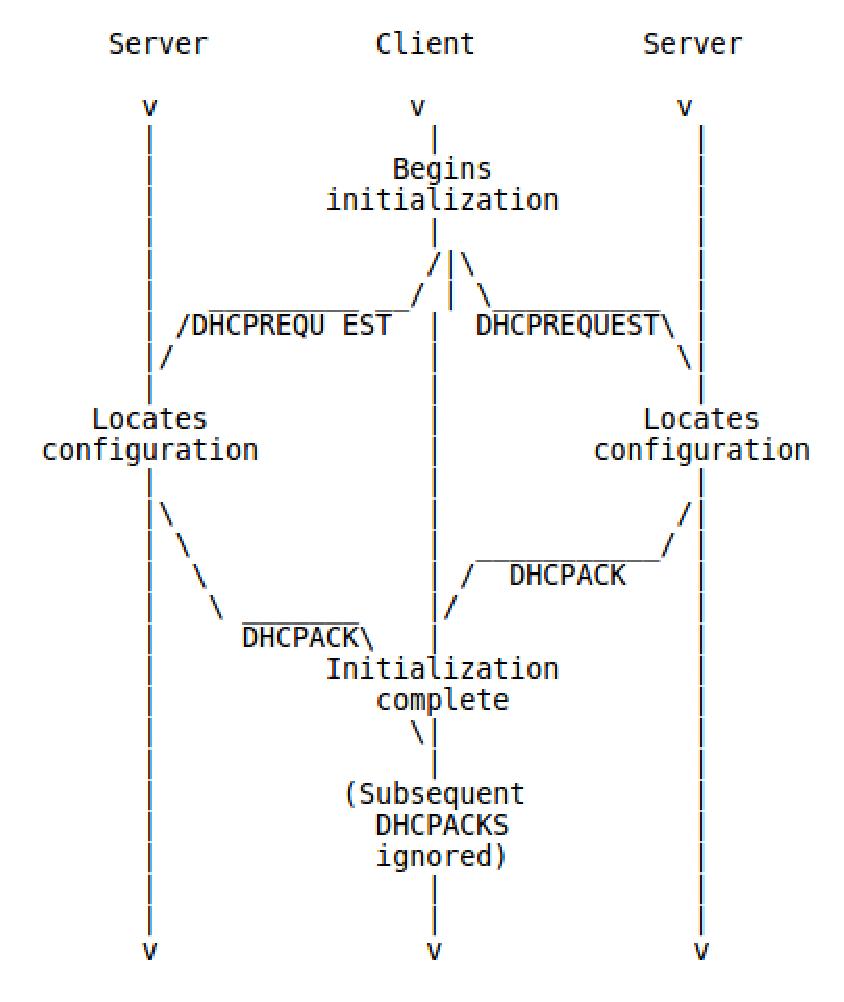
\includegraphics[width=6cm]{./pics/timeline_dhcp_reuse_add.eps}
\caption{Déroulement de la négociation DHCP pour la réutilisation d'une configuration}
\label{fig:timelinedhcpreuseadd}
\end{figure}

%---------------------------------------------------------------------------------

\subsection{PMTU discovery}
Le protocole PMTU discovery (Path MTU discovery) décrit dans le RFC
1191\cite{url-RFC-PMTU}, permet de trouver le plus petit MTU d'un chemin entre
l'émetteur et le récepteur. Cela permet d'éviter la fragmentation des paquets
IP ce qui permet entre autre de soulager la charge des routeurs.  L'hôte
souhaitant connaître le plus petit MTU pour un chemin vers autre hôte va
envoyer un paquet avec un certain MTU et en plaçant le bit DF de l'entête sur 1
pour éviter la fragmentation du paquet. Ainsi si le MTU est trop grand à un
moment donné du chemin, le routeur ne pourra pas fragmenter le paquet mais ne
pourra non plus pas transmettre le paquet en l'état. Il va alors détruire le
paquet, et émettre un message ICMP de type 3 et de code 4 vers la source du
paquet, signalant que la destination n'est pas joignable, et que cela est dut à
un paquet nécessitant une fragmentation or celle-ci est interdite. Le MTU est
donc trop élevé. Le message ICMP contient le MTU qu'il faut passé le routeur.
L'émetteur va alors créer un nouveau paquet avec le nouveau MTU. Il fera cela
autant de fois que cela est nécessaire pour déterminer le MTU du chemin.

\subsection{DNS}
Le protocole DNS (Domain Name System) permet de faire de la résolution
d'adresse.  Cela est permis grâce à des échanges avec un ou plusieurs serveur DNS.
Un serveur DNS va faire de la traduction de nom de domaine, notamment en adresse IP. Pour
simplifier, le nom de domaine, facilement retenu par un être humain va être
traduit en adresse IP pour être utilisée par l'ordinateur.  Nous n'aborderons
pas plus le fonctionnement de DNS car s'est un protocole de couche application
et qu'il n'est pas essentiel au fonctionnement d'IPv4. Cependant il reste
essentiel dans l'utilisation d'Internet, aujourd'hui, par des êtres humains.

\section{Passage de IPv4 à IPv6}
\subsection{Raison du passage de IPv4 à IPv6}
\subsubsection{Problème posé par IPv4}
//Pénrurie, adressage privé/publique compliqué
% Il se trouve que apparement il y a des problemes de
% penurie d'adresses meme dans certaines reseau prive`
% http://blog.erratasec.com/2013/12/dod-address-space-its-not-conspiracy.html#.WAf_d7Wf21F

PROBLÈMES DE IPV4

ÉPUISEMENT DES ADRESSES
Lorsque IPV4 a été développé dans les années 70-début des années 80, personnes n'aurait imaginé qu'il y aurait un jour autant d'interfaces qui se connectent à Internet. On pensait qu'une adresse sur 32 bits serait suffisante. De plus, les plages d'adresses étaient distribuées généreusement au début. Cela veut dire que l'on attribuait des adresses permettant un nombre d'interfaces beaucoup plus grand que nécessaire.
Cependant, avec la croissance du nombre d'utilisateurs, la plage d'adresses IPV4 disponible a diminué progressivement. C'est en février 2011 que la réserve de bloc libres d'adresses publics IPV4 de l'IANA (Internet Assigned Numbers Authority) est arrivée à épuisement.
Afin de résoudre ce problème, plusieurs techniques ont été proposées.
La première a été le changement de teechnique d'adressage. On est passé de la technique de classe d'adressage IP à la technique Classless Inter-Domain Routing. Ceci à permis une meilleure efficacité dans la distribution des adresses IP grâce à la création de réseau de tailles intermédiaire. En effet, avant on ne disposait que de réseau de 3 tailles différentes.
Les politiques d'assignement d'adresses ont également été rendu plus stricte afin de mieux tenir compte des besoin réels des demandeurs d'adresses IP.
Il a aussi été décidé d'utiliser des blocs autrefois réservé comme 14.0.0.0.
Sur base de volontarisme, des blocs autrefois attribués généreusement ou alors des IP non utilisées ont été récupérées. 
Finalement, il a été remarqué qu'il n'était pas nécessaire que chaque interface a son adresse IP public et le protocole NAT a été développé afin de regrouper plusieurs interface sous une même adresse IP. Ce protocole est de plus en plus utilisé dans IPV4 depuis la fin des années 90.

Fonctionnement du NAT dynamique (Network Adress Translation)
Le NAT est une technique utilisée au niveau du routeur. Le principe du NAT est
que le routeur fait correspondre à une adresse IP une autre adresse IP. En
général cette technique est utilisée pour avoir une même adresse IP pour tout
un réseau comme un intranet ou encore un réseau domestique. Dans ce réseau,
toutes les interfaces - même le routeur - auront une adresse privée. Le routeur
dispose en plus de cela de une ou plusieurs adresses publics avec lesquelles il
est connecté à internet. Une adresse privée est une adresse qui est utilisée à
l'intérieur d'un réseau local. Les adresses privées peuvent être choisies parmi
les suivantes: 10.0.0.0/8, 172.16.0.0/12 ou 192.168.0.0/16.  Lorsqu'une
interface envoie un paquet vers l'extérieur du réseau, le routeur effectue
plusieurs changements. Il traduit d'abord l'adresse privée en adresse public et
la met dans l'en-tête du paquet. Puis il change tous les checksums qui tiennent
compte de l'adresse IP. Enfin, il garde en mémoire dans une table la
correspondance entre adresse privée/adresse public comme ci-dessous.  <tableau
adresse public / privée >
Cela n'est cependant pas suffisant. En effet, lorsqu'un paquet arrivera de l'extérieur du réseau,  et si tous les interfaces utilisent la même adresse public sans distinction supplémentaire, le routeur ne saura pas à quelle interface envoyer le paquet. 
Une solution à ce problème existe pour les protocoles utilisant les ports comme TCP et UDP. Le routeur ajoute une information supplémentaire dans la table qui est le port source d'où vient le paquet. Les ports, qui sont implémentés dans la couche transport (couche 4), sont des sortes de ''portes'' qui permettent de communiquer avec un système d'exploitation. Le numéro de port est un numéro choisit aléatoirement entre 1024 et 65535.
Pour illustrer le fonctionnement du NAT imaginons qu'une interface A dont l'ip est 192.168.0.1 veut envoyer un paquet à l'interface B d'ip 217.70.184.38. Le port source est le port 10277 et le port destination est le port 80. 
La table NAT ressemblera à ceci:

<TABLE NAT complète > 

La box internet enverra le paquet:

L'interface B répondra en envoyant le paquet:

Lorsque la box reçoit ce paquet, elle voit que le port de destination est le port 10277. Elle cherche ensuite le port correspondant dans sa table NAT. Lorsqu'elle le trouve elle effectue les changements nécessaire sur le paquet et transmet le paquet à l'interface A.
Mais même si cette solution fonctionne la plupart du temps, la probabilité est faible que 2 interfaces envoient des paquet sur les même port. C'est pour éviter cela que la box change le port source lorsqu'elle reçoit un paquet de l'interface A. Ainsi on s'assure que aucun port n'est utilisé plusieurs fois. Enfin, pour éviter de saturer les ports utilisés, un compteur est associé à chaque paire adresse public/adresse privée. Lorsqu'il n'y a pas de trafic entre une adresse privée et l'extérieur durant une durée fixée, le port qui lui est associée peut être réutilisé pour une autre adresse privée.

Le NAT dynamique apporte cependant un grand problème. Lorsqu'une interface
extérieur veut se connecter à une interface dans le réseau, elle ne dispose
d'aucune autre information que l'adresse IP public. Si elle envoie alors un
paquet à cette adresse, le routeur qui le réceptionnera ne saura pas quoi faire
avec et le paquet sera perdu.  On a réussi à pallier à ce problème grâce au
port forwarding. 

PORT FORWARDING

NAT STATIQUE


\subsubsection{Solutions}
//NAT,IPv6
\subsection{Différence entre IPv4 et IPv6}


\section{Conclusion}

Pour conclure, l'iPv4 est un protocole réseau (couche 3 du modèle OSI) qui
 a été développé dans les années 70. Les objectifs lors de son développement 
étaient d'obtenir un protocole réseau qui permet une communication efficace sur, et entre 
plusieurs réseaux informatiques. C'est un protocole basé sur la commutation de paquets, ce 
qui permet d'établir de nombreuses connexions simultanément alors qu'avant, notamment dans les réseaux téléphoniques, une connexion utilisait le lien à elle seule. 
\\
Même si des protocoles réseau existaient déjà auparavant, IPv4 a apporté une standardisation ainsi
que la commutation par paquet qui ont permit la diffusion d'internet à grande échelle.
\\
L'un des objets centraux de l'IPv4 est l'adresse IP. Elle est composée de 4 nombres allant de 0 à 255 
grâce auxquels on obtient une adresse IP écrite de cette façon : 255.0.24.35 .
C'est avec cette adresse que les interfaces/routeurs s'identifient sur internet de façon unique 
lorsqu'elle sont publiques ou de façon unique sur le réseau dans lequel elle se trouve lorsqu'elles sont locales. 
C'est donc également elle qu'on manipule pour trouver/identifier des interfaces sur le réseau/internet.
 Sa forme est restée la même au cours du temps mais la façon dont elle est allouée a été modifiée.
Il existe plusieurs types d'adresses qui sont les adresses unicast, multicast, anycast et broadcast.
 Chacune d'entre elle permet d'atteindre une ou plusieurs interfaces en fonction de certains
critères. Certaines adresses/ plages d'adresses sont également réservées pour des usages spéciaux. 
Un avantage important d'IPv4 est également la configuration automatique qui permet la mise 
en place d'un réseau sans connaissances techniques.
\\
Le second objet central d'IPv4 est le paquet IP. Un paquet est l'unité d'information réseau, donc 
de niveau 3, dans lequel sont mises les informations à transmettre. Un paquet est divisé en 2 
parties : l'en-tête et une partie donnée dans laquelle sont mises les informations à envoyer.
 L'en-tête d'un paquet IP est mis au début de ce dernier. Il donne des informations aux 
routeurs et interfaces par lesquels il transite afin d'arriver à la bonne destination. Les
 informations qui y sont contenues sont nombreuses: le protocole réseau utilisé (4 dans le
 cas d'IPv4), la taille de l'en-tête, la taille totale du paquet, un identificateur de 
fragments de même paquet, un fragment offset pour retrouver la place d'un fragment dans 
un paquet reconstitué, la durée de vie qui indique en pratique le nombre de sauts que 
peut faire un paquet IPv4, l'adresse source, l'adresse de destination et d'autres encore.
\\
Enfin, de nombreux protocoles ont été définis afin de garantir le bon fonctionnement des
 adresses IPv4. Certains protocoles servent à contrôler l'intégrité des adresses IPv4. L'ACD permet par exemple de garantir l'intégrité d'une adresse en détectant l'utilisation
de la même adresse IP par deux ou plusieurs hôtes en même temps. 
L'ICMP quant à elle permet de faire des contrôles d'erreurs et des vérifications.
D'autres permettent d'utiliser des fonctionnalités comme le protocole IGMP qui permet aux 
interfaces de s'abonner a des groupes multicast ou encore le protocole DHCP qui permet 
l'auto-configuration des interfaces. D'autres protocoles permettent finalement de simplifier
 ou de rendre plus efficace  l'utilisation d'internet comme les serveurs DNS qui font la
 traduction entre nom de domaine, comme Google.fr, et son adresse IP ou encore le PMTU 
discovery qui permet d'éviter la fragmentation de paquets.
\\
Cependant, même si au début IPv4 a été conforme aux attentes, internet a grandit de façon
 exponentielle et des problèmes auxquels ne s'attendaient pas ses concepteurs sont apparus.
Le problème le plus important d'entre eux a été l'épuisement d'adresse. En effet, internet n'était 
initialement pas destiné a un usage si répandu mais uniquement à un usage militaire et scientifique. 
Ainsi, à force de se répandre les plages d'adresses disponible s'amenuisèrent rapidement
 et c'est en février 2011 que la réserve de bloc d'adresses publiques libres IPv4 de
 l'IANA (Internet Assigned 
Numbers Authority) est arrivée à épuisement. Des techniques de contournement ont donc été
 inventées.  La plus simple a été la récupération de plages d'adresses. Une autre a été une
 modification dans l'adressage d'IPv4 en passant de la méthode classfull network à la
 méthode classless network. Ceci a permit d'éviter de gaspiller de nombreuses adresses
 IP. Enfin, à travers la traduction d'adresse (NAT : Network Adress Translation), de
 nombreuses interfaces ont pu être rassemblées sous une même adresse IP. Ainsi, on a pu
 retarder l'épuisement des adresses IP mais on n'a pas réglé le problème.
\\
Ensuite, il y a également eu d'autres problèmes plus petit concernant la sécurité et la performance qui n'étaient pas directement intégrés dans IPv4. 
\\
C'est pour cela que l'IETF a décidé dans les années 90 de travailler sur un nouveau protocole 
réseau qui répondra mieux aux besoins de l'Internet d'aujourd'hui. Ce nouveau protocole qui se nomme
IPv6 ainsi que son environnement ont été développé dans les années 90 et publié en 1998
 dans le RFC2460. Il apporte un espace d'adressage sur 128 bits, ce qui régla tous les soucis
 concernant l'épuisement de ce dernier. 
En plus de cela il amène une amélioration au niveau de la sécurité avec l'intégration de protocole
 tel que IPsec qui en devient partie intégrante alors qu'il n'était qu'optionnel dans IPv4. Enfin,
 IPv6 amène des améliorations au niveau des performances avec l'élimination du NAT qui enlève une
 couche supplémentaire, une simplification de l'en-tête du paquet ainsi qu'une diminution des
 traitements effectués par les routeur grâce à la fragmentation au niveau de l'émetteur et le déplacement des
 checksums dans les protocoles de niveau 4.

C'est à cause de tous ces avantages que l'IPv6 a été développé afin de remplacer l'IPv4. 
Cependant, la migration qui se déroule actuellement est lente et difficile. En effet, il 
faut faire cohabiter ces deux technologies, ce qui peut mener à des soucis de sécurité. Enfin, au 
début de 2016, le déploiement IPv6 est encore très limité car la proportion d'utilisateurs Internet en
 IPv6 est estimée à 10\%. Il faudra donc encore longtemps avant que tous les utilisateurs d'internet 
sont passés à IPv6.






\addcontentsline{toc}{section}{Références}
\bibliographystyle{plain}
\bibliography{rapport}

\end{document}
